\documentclass[onecolumn, draftclsnofoot,10pt, compsoc]{IEEEtran}

\usepackage{float}
\usepackage{graphicx}
\usepackage{url}
\usepackage{setspace}
\usepackage{geometry}
\usepackage{listings}
\usepackage{color}
\usepackage{etoolbox}
\usepackage{pdflscape}

\patchcmd{\thebibliography}{\section*{\refname}}{}{}{}

\geometry{textheight=9.5in, textwidth=7in}

% 1. Fill in these details
\def \CapstoneTeamName{			              			 PlanteR-GB}
\def \CapstoneTeamNumber{					           			 Group 64}
\def \GroupMemberOne{				           				Austin Hodgin}
\def \GroupMemberTwo{				           				Travis Hodgin}
\def \GroupMemberThree{			            Maximillian Schmidt}
\def\GroupMemberFour{		        	               Zach Lerew}
\def \CapstoneProjectName{	      	    Winter is Coming...}
\def \CapstoneSponsorCompany{		    Oregon State University}
\def \CapstoneSponsorPerson{		 			  				 Victor Hsu}

% 2. Uncomment the appropriate line below so that the document type works
\def \DocType{
	%Problem Statement
	%Requirements Document
	%Technology Review
	%Design Document
	Final Progress Report
}

\newcommand{\NameSigPair}[1]{\par
\makebox[2.75in][r]{#1} \hfil 	\makebox[3.25in]{\makebox[2.25in]{\hrulefill} \hfill		\makebox[.75in]{\hrulefill}}
\par\vspace{-12pt} \textit{\tiny\noindent
\makebox[2.75in]{} \hfil		\makebox[3.25in]{\makebox[2.25in][r]{Signature} \hfill	\makebox[.75in][r]{Date}}}}
% 3. If the document is not to be signed, uncomment the RENEWcommand below
\renewcommand{\NameSigPair}[1]{#1}

%%%%%%%%%%%%%%%%%%%%%%%%%%%%%%%%%%%%%%%
\begin{document}
\begin{titlepage}
    \pagenumbering{gobble}
    \begin{singlespace}
    	%\includegraphics[height=4cm]{coe_v_spot1}
        \hfill

        % 4. If you have a logo, use this includegraphics command to put it on the coversheet.
        
\includegraphics[height=4cm]{logo.png}

        \par\vspace{.2in}
        \centering
        \scshape{
            \huge CS Capstone \DocType \par
            {\large\today}\par
            \vspace{.5in}
            \textbf{\Huge\CapstoneProjectName}\par

            %\vfill
			\vspace{1in}

            {\large Prepared for}\par
            \Huge \CapstoneSponsorCompany\par
            \vspace{5pt}
            {\Large\NameSigPair{\CapstoneSponsorPerson}\par}

			\vspace{1in}

            {\large Prepared by}\par
						{\huge \CapstoneTeamNumber}\par
            \CapstoneTeamName\par
            \vspace{5pt}

            {
				\Large
				\NameSigPair{\GroupMemberOne}\par
				\NameSigPair{\GroupMemberTwo}\par
				\NameSigPair{\GroupMemberThree}\par
				\NameSigPair{\GroupMemberFour}\par
            }

            \vspace{20pt}
        }
				\newpage
        \begin{abstract}
				\noindent This is the abstract for the WHOLE paper.
        \end{abstract}
    \end{singlespace}
\end{titlepage}

\newpage

\pagenumbering{arabic}
\tableofcontents
% 7. uncomment this (if applicable). Consider adding a page break.
\listoffigures
%\listoftables
\clearpage
\singlespace

\newpage


% Syntax highlighting
\definecolor{mygreen}{rgb}{0,0.6,0}
\definecolor{mygray}{rgb}{0.5,0.5,0.5}
\definecolor{mymauve}{rgb}{0.58,0,0.82}

\lstset{
	backgroundcolor=\color{white},   % choose the background color
	basicstyle=\footnotesize,        % size of fonts used for the code
	breaklines=true,                 % automatic line breaking only at whitespace
	captionpos=b,                    % sets the caption-position to bottom
	commentstyle=\color{mygreen},    % comment style
	escapeinside={\%*}{*)},          % if you want to add LTeX within your code
	keywordstyle=\color{blue},       % keyword style
	stringstyle=\color{mymauve},     % string literal style
	frame = single,                  % code framing
}


	Hello \cite{expensive1}
	

	\section{Introduction} % Include information to answer these questions in the problem statement:
	% Who requested it?
	% Why was it requested?
	% What is its importance?
	% Who was/were your client(s)?
	% Who are the members of your team?
	% What were their roles?
	% What was the role of the client(s)? (I.e., did they supervise only, or did they participate in doing development)
		\section*{Problem Description}
	During the cold and dark winter months, plant growth becomes difficult at best, and calamitous at worst. In our state of Oregon we are well accustomed to overcast, low temperatures, and rain throughout the winter, spring, and fall months. Our client has a desire to grow herbs and plants indoors during these long, cold months. Solving this problem is a desire held by all members of our team. Much like our client, we enjoy cooking with fresh herbs and vegetables even through the winter.
	\\\\Many plants and herbs such as tomatoes, basil, ferns, and plants from foreign climates have an ideal set of environmental conditions that allow for optimum growth. Variables such as light wavelength, intensity, temperature, moisture, and pests all have an impact on a plant's health and yield. These factors lead many growers to bring their plants indoors during the winter months.
	\\\\Even in a climate controlled dwelling, the problem persists. Humans and plants require very different living conditions. Residents come and go from work, school, and vacation while plants have evolved to expect the 24hr day-night cycle. Busy humans can leave plants neglected or without light for days. Current interior plant lighting systems can be expensive and offer little to no customization. Plant growth systems that do not adapt to both the requirements of their plants and their gardener's schedule lead to frustration, low plant yield, and plant death.

	\section*{Proposed Solution}
	The client's primary concern is solving the problem of interior plant lighting. The features required to do this are clearly defined in the \textit{required features} section, but specific implementation details were left to our team. Each of us have skills in an area related to this project, and together we have the ability to go above and beyond what was requested by the client. We have built the set of \textit{additional features} listed below that we believe compliment the client's vision for this project.
	\\\\ Given proper design and documentation, the additional features are likely to be completed barring any complications. Features that are especially difficult to accomplish, unlikely to be completed, or are outside the primary scope of the project are listed as \textit{stretch goals}.

	\subsection*{Required features - v1.0}
	\begin{itemize}
		\item LED lighting for a single plant bed
		\begin{itemize}
			\item A simple LED strip with a single controller attached to a single planter
			\item Service running on a micro controller that can control the power state of attached LED lights
			\item Configuration settings for the light state is read from a configuration file
			\item Changes to the configuration file are recognized and applied by the controller
		\end{itemize}
		\item Color and intensity Control
			\begin{itemize}
				\item User can select the color and light intensity of the light strip
			\end{itemize}
		\item Lighting state schedule
			\begin{itemize}
				\item User can specify weekly and daily scheduling for the state of the light (Color, Intensity, Power)
			\end{itemize}
		\item Zoning for individual control over multiple strips
			\begin{itemize}
				\item Controller supports individual control of up to 20 zones
				\item Each zone can chain light strips together on one data pin
			\end{itemize}
		\item Simple user interface for basic control
			\begin{itemize}
				\item Simple interface to edit configuration settings and physically transfer changes to the controller
				\item All settings can be changed from this interface, though it may not be user friendly
				\item Controller recognizes configuration changes and applies them automatically
			\end{itemize}
	\end{itemize}

	\subsection*{Additional features - v2.0}
	\begin{itemize}
		\item Improved User Interface
		\begin{itemize}
			\item Hosted web interface on local network
			\item Easy to use and responsive interface that shows the current state of the system
			\item All system settings can be updated and applied over the network without the need for physical access to the controller
		\end{itemize}
		\item Sub zoning on an individual light strip
			\begin{itemize}
				\item Multiple colors and intensities on a single light strip using LED indexing
			\end{itemize}
		\item Flexible zoning and sub-zoning
			\begin{itemize}
				\item Whole light strips and sub strips can be zoned together for more precise lighting control
			\end{itemize}
		\item Mobile web interface
			\begin{itemize}
				\item Web interface adds mobile support
				\item Android application acting as a wrapper for the web interface
			\end{itemize}
		\item Custom enclosure with vertical lighting
			\begin{itemize}
				\item Custom designed planter that holds the controller and lights
			\end{itemize}
		\item Environmental monitoring
			\begin{itemize}
				\item Monitoring for humidity and temperature using additional hardware sensors
				\item Web interface plugin to monitor humidity and temperature
			\end{itemize}
	\end{itemize}

	\subsection*{Stretch goals - v3.0}
	\begin{itemize}
		\item Modular light strips and enclosure
			\begin{itemize}
				\item Easy to attach light strips are automatically detected and setup
				\item Snap together enclosures allow quick and effortless system control
			\end{itemize}
		\item Gardening guide built into interface to help user learn best gardening practices
			\begin{itemize}
				\item Interface provides tips and suggestions to improve growing and gardening
			\end{itemize}
		\item Modular planting enclosure with snap together components
			\begin{itemize}
				\item Self contained enclosures with plug-and-play connectors for automatic and hassle free setup of multiple planters
			\end{itemize}
		\item Irrigation system
			\begin{itemize}
				\item Hardware and software necessary to facilitate automatic or scheduled watering
				\item *Requires custom enclosure
			\end{itemize}
		\item Wireless control over multiple plant growth systems
			\begin{itemize}
				\item Ad hoc style wireless system to allow seamless control over multiple grow light systems
				\item Support for large distributed systems, such as greenhouses
			\end{itemize}
	\end{itemize}

	\section*{Performance Metrics}
	Defining performance metrics for this project has been a back and forth topic for this team. The client's requirements are easily met by a team of four people, but our internal expectations are much higher. To avoid feature bloat and to guarantee the product functions per the client's requirements at a minimum, the features below describe the features necessary to define the project as a success. Extra features will be added after the completion of these functionally required features.
	\begin{itemize}
		\item \textbf{All features described by the client} listed in section \textit{Required features} are complete.
		\item An alternative interface as described in \textit{Additional features}. An interface that allows all controller settings to be modified without \textit{physical access to the controller}.
		\begin{itemize}
			\item This interface will likely be a web server hosted on the controller, but is subject to change as the project evolves.
		\end{itemize}
	\end{itemize}


	\section{Requirements Document}
	% Add (your client should have okay'd): What new requirements were added? What existing requirements were changed?
	% What existing requirements were deleted? Why? 
	% Add: Final Gantt Chart as a record of what happened when.
		\section{Introduction}

		\subsection{Purpose}
			The goal of this document is to clearly list and define each of the requirements defined by the client.  Looking ahead, this will refine what the end result of the project shall be,
			such that the client's and team's expectations are fully met after all work is completed.  This document will also address any uncertainty about the end result of the proposed product,
			before work begins.
		\subsection{Scope}
			This document represents the set of requirements initially provided by the client as interpreted by the development team, and successive additions created to improve upon the client's initial feature set.
			Such requirements will mold the final product in its form and functionality. To detail each requirement, the team has provided technical specifics on how each requirement will be met.  The document also
			includes the details that the team will be executing step by step	during the project to meet said result.

		\subsection{Definitions, Acronyms, and Abbreviations}
			LED - Light Emitting Diode
			\\RGB - Red, Green, Blue. Usually referring to a LED that is capable of producing those three colors.
			\\GPIO - General Purpose Input Output pins, allow the transfer of data between a microcontroller and an external piece of hardware.
			\\TCP - Transmission Control Protocol
			\\UDP - User Datagram Protocol
			\\REST - Representational state transfer
			\\API - Application Programming Interface


		\subsection{Overview}
			In accordance with the requirements laid out by the client and team, an overall description has been provided that will detail the specifics on what will be used. Version numbers, as well as internal iterations of the versions, will detail
			and divide each set of specifications and the application of the mentioned software and hardware.


	\section{Overall Description}
		\subsection{Product Perspective}

		\subsubsection{Product Functions}
		\noindent \textbf{Version 1.0} will consist of three major parts. The first part will be the programmable LEDs that will be used to light the plants. These will need to be reprogrammable in order to allow new settings.
		These settings include LED color on the RGB spectrum, intensity of the light, and the time the LEDs will turn on, and turn off. All LEDs in this version will be set to the same settings, meaning all
		LEDs will have the same color, intensity and light time. The second part will be the microcontroller. The microcontroller will allow the LEDs to be programed, and will provide power for early iterations.
		The third part is a user interface to allow these settings to be changed. This version will consist of a configuration file that can be manually changed to modify these settings.

		\noindent \textbf{Version 2.0} consists of additional features added by our team. Version 2.0 will require everything from Version 1.0 to be completed. This version will add many new features. The first, and most
		important feature will be an easier way to manage the settings. This version will add a web interface that will allow the user to change settings without having physical access to the controller.
		This new user interface will be able to display the current settings as well as allow the user to make changes. Further additions to the user interface include adding a mobile web page, and native mobile application for
		phone support to allow users to update settings on their phone or other mobile device, further adding easier access to the settings. This version will also allow the user to change the LEDs to a new color or intensity for more flexibility. Adding moisture and temperature sensors is another goal for this version. Adding these will further allow the user to adjust
		their environment for the specific plants they are growing.

		\noindent \textbf{Version 3.0} consists of our stretch goals: goals that we will attempt to complete when we are finished with version 1.0 and 2.0, given we have enough time. This version, like the last version,
		requires all previous versions to be complete. Our first stretch goal will be to add predefined setting profiles for various plants. These include adding color, intensity and light timings optimized
		for various types of herbs, such as parsley vs basil. This further makes settings easier to manage for the user, taking much of the guess work or research out of the equation. Another stretch goal will be
		to add modular planter boxes. This goal intends to allow the user to add planters together using a single microcontroller. Further goals include to expand this set up to larger scale growing systems,
		such as greenhouses.


		\subsubsection{System Interfaces}
				The system as a whole serves as an arbitrator between a user and the ideal growth of their plants.
				The microcontroller will have control over a series of LEDs, including their color, intensity, and power schedule. The same microcontroller will host an interface that allows the user to control
				how the microcontroller adjusts the properties of its LEDs. Initially during iteration zero and one, the user interface to the system will be simplistic and require a high skill ceiling to use. As the project matures into iteration six, a more useful and
				simplistic interface will be developed. Similarly, the number of supported LEDs will be limited until iteration five when a better power management solution is made.
		 \subsubsection{User Interfaces}
				System properties will be controlled through a configuration file that is read by the control service and transformed into the appropriate GPIO signals to change the LED state. Starting at
				iteration one, the configuration file will be the primary and only way to interact with the system's properties. After core abilities are developed, iteration two will create a text-based command
				line menu system that allows all settings to be modified. This command line menu will be updated until iteration five, after which it will be replaced.
				The iteration six web interface will be hosted on the microcontroller and will communicate with the control service through changes to the configuration file. This interface will be clearly
				organized into categories for each of the major features (e.g. Zones, Scheduling, Profiles, manual control, etc).
			\subsubsection{Hardware}
				The microcontroller will be the brains for this system, and needs to be capable of running a service that controls the LEDs, as well as hosting a web server accessible from the local network.
				For iteration zero, the microcontroller must be capable of delivering enough power for a single LED strip. Iteration five will use a separate power supply, but the microcontroller must still control
				at least four LED strips. Iterations twelve and fifteen will require a separate power supply and regulator chip and possibly support data over USB to support larger lighting systems.
			\subsubsection{Software Interfaces}
				The control service is the bridge between the LEDs and the user interface, it will run on a microcontroller as a background service.
				In version 1.0, the user interface will be simplistic but functional. There will be a higher barrier of entry required to use these early interfaces, to allow the project to focus on the primary features of the system.
				After iteration five, a web interface will be developed. It will be hosted using a website hosting service such as Apache2. The web interface will use a simple tabular card based interface
				that will allow all system settings to be viewed and modified as the system is running.

			\subsubsection{Communications Interfaces}
				The control service will communicate with LEDs over the microcontroller's GPIO pins. Data transfer to the LEDs will occur over GPIO pins until iteration thirteen and higher which can bring support for a
				large amount of LEDs, but may require communication over USB.
				Iteration thirteen will bring support for communication between distributed systems over the TCP through a REST API built into the control service.
			\subsubsection{Memory Constraints}
				The memory constraints are determined by the type of programmable LED chosen and the type of microcontroller. Memory constraints will change as parts are specified and become part of the project.

			\subsubsection{Operations}
				The operations of this product change based on which iteration we are on. In the first iteration the user will be operating the system through a configuration file on the system. In the second iteration
				the way the user interacts with it changes to an interactive script. This script will ask questions about how the user would like to configure the system, then makes the changes to the configuration file to configure the system.
				The sixth iteration will then change the user operations again by allowing the user to make configurations using a web interface hosted by the system. With each step the system will apply changes from the configuration file
				in a steady interval (Instant, 5 sec, 10 sec, 30 sec). This is subject to change based on how long the control service takes to reload and apply the changes.
			\subsubsection{Site Adaptation Requirements}
				The system will change to support different number of LEDs, which are limited by software, depending on which iteration we are in. With iteration four, two zones will be controlled and powered by the microcontroller.
				In iteration five the amount of zone will increase to four zones powered by a separate power supply. With iterations twelve and fifteen another controller may be needed to push settings to the increased number of LEDs.


		\subsection{User Characteristics}
		Iterations zero and one will require the user to connect to the microcontroller, either physically, or through an SSH/FTP connection. Knowledge on how to traverse common folder systems will be needed for physical transfer, such as
		through an SD card or USB connection. SSH connections will require the user to know how to traverse a Unix terminal.
		Iteration two through five will require the user to know how to traverse a Unix terminal, as well as run a script. Users will further have to follow a list of questions and answer them with correct color, intensity, and time.
		Iteration five through fifteen will require the user to be able to connect to a website hosted by the microcontroller by connecting to its local host. The user will also need to know how to click buttons and go through drop down menus on the site.

		\subsection{Constraints}
		For iterations zero through four, we will be constrained to using only a max of ten LEDs, due to power limitations, the limitation of the number LEDS is an estimation based on the power outputs various microcontrollers. For iterations five through ten, we will be constrained to powering the LEDs off a separate power supply than the microcontroller,
		since we may be using more than the max for iterations zero through four. We will have more constraints based on the microcontroller used. Certain controller will have more or less GPIO pins. Microcontrollers may have different clock speeds, and RAM sizes.

		\subsection{Assumptions and Dependencies}
		Each version and iteration requires that the previous versions and iterations be complete. Version 2.0 requires version 1.0 to be finished, and iteration five requires that iteration zero through four be finished.
		Through iteration five and onward, we will be working with more LEDs. Depending on the microcontroller, the LEDs may need to be powered separately from the controller itself, as they may draw too much current.
		Iteration twelve through fifteen will depend on a separate LED controller that will help facilitate the indexing of, and controlling of the LEDs. This also depends on the availability of such a controller.

		\newpage
		\begin{landscape}
		\subsection{Gantt Chart}
		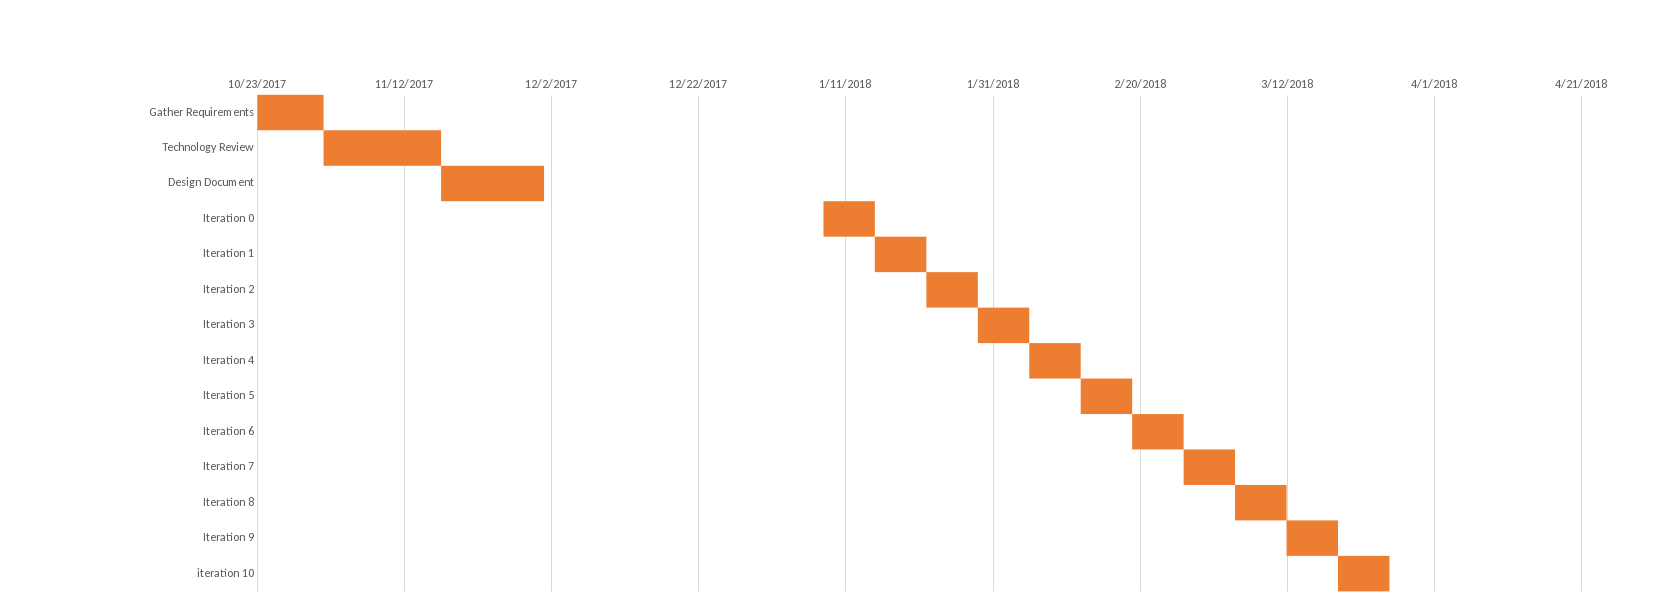
\includegraphics[width=\linewidth]{Gant.png}
		\end{landscape}
		\newpage


	\section{Specific Requirements}
		\subsection{Required features - v1.0}
			\begin{itemize}
				\item Iteration 0
						\begin{itemize}
						\item A single LED strip with a single microcontroller intended to be used with a single planter
						\item Background service running on microcontroller which can communicate with LEDs through GPIO pins
						\item Control light color and intensity
					\end{itemize}
						\item Iteration 1
					\begin{itemize}
						\item Configuration settings for the light state is read from a configuration file
						\item Changes to the configuration file are recognized and applied by the controller at a regular interval
					\end{itemize}

				\item Iteration 2
					\begin{itemize}
						\item Simple user interface using command line script for basic control over settings
						\item All settings can be changed from this interface, though it may not be user friendly
					\end{itemize}
				\item Iteration 3
					\begin{itemize}
						\item User can specify weekly and daily scheduling for the state of the light (Color, Intensity, Power)
					\end{itemize}
				\item Iteration 4
					\begin{itemize}
						\item Light zoning - zones can be controlled and scheduled individually
						\item At least two zones supported and powered by microcontroller
					\end{itemize}
				\item Iteration 5
					\begin{itemize}
						\item Controller supports at least four and at most 20 zones, powered separately from the microcontroller
						\item Each zone can chain light strips together on one data pin due to strips being powered separately
					\end{itemize}
			\end{itemize}

		\subsection{Additional features - v2.0}
			\begin{itemize}
				\item Iteration 6
					\begin{itemize}
						\item Hosted web interface on local network
						\item Interface remains as simple as possible
						\item Shows the current state of the system
						\item Can modify all configuration settings of control service on local microcontroller
					\end{itemize}
				\item Iteration 7
					\begin{itemize}
						\item Sub zoning on an individual light strip
						\item Color and intensity set per LED
						\item LEDs grouped into zones, regardless of which strip they are on
					\end{itemize}
				\item Iteration 8
					\begin{itemize}
						\item Web interface adds support for mobile sized screens
						\item Native mobile application acting as a wrapper for the web interface
					\end{itemize}
				\item Iteration 9
					\begin{itemize}
						\item Custom 3D printed planter with enclosure for controller, power supply, and LEDs
					\end{itemize}
				\item Iteration 10
					\begin{itemize}
						\item Humidity and temperature monitoring using additional hardware sensors
						\item Web interface support for humidity and temperature logging
					\end{itemize}
			\end{itemize}

		\subsection{Stretch goals - v3.0}
			\begin{itemize}
				\item Iteration 11
					\begin{itemize}
						\item Pre-built profile settings and per-plant settings that allow effortless light configurations to be applied that are specific to a particular plant species
					\end{itemize}
				\item Iteration 12
					\begin{itemize}
						\item Custom printed modular enclosure that allows multiple planters to be snapped together under a single controller
						\item Lights are automatically detected and zoned
					\end{itemize}
				\item Iteration 13
					\begin{itemize}
						\item Wireless “ad-hoc” style control over multiple distributed systems
						\item Control service will take input from a network protocol, allowing the web service to be run on a different local machine
					\end{itemize}
				\item Iteration 14
					\begin{itemize}
						\item Pre-setup OS/lighting system image for microcontroller, instruction guide for building your own system
						\item Kit with all necessary parts, pre-flashed system image
						\item Pre-built kit, plug and play, sold for profit
					\end{itemize}
				\item Iteration 15
					\begin{itemize}
						\item Support for very large distributed systems such as greenhouses
					\end{itemize}
			\end{itemize}

		\section{Performance Metrics}
		Defining performance metrics for this project has been a back and forth topic for this team. The client's requirements are easily met by a team of four people, but we have set our internal expectations are much higher. To avoid feature bloat and to guarantee the product functions per the client's requirements at a minimum, the features necessary to describe the project a success are a smaller subset of the overall features described in this document. This project is considered a success if: All features described in Version 1.0 are completed per specification and an alternative interface as described in iteration six is completed. Extra features will be added after the completion of these required
		features.


	\section{Design Document}
	% Add (your client should have okay'd): What design aspects were changed, deleted or added? Why?
		\section{Introduction}

		\subsection{Purpose}
		The aim of this document is to provide a solid base that the implementation of the system can build upon. It generalizes how the RGB LEDs system
		operates, yet details how each researched technology contributes to the overall function. The specifics of the implementation may change as new
		challenges are presented, but the overall system function and design should not.

		\subsection{Scope}
		Due to the minimal requirements set on the project, the core design only covers items up until the end of Iteration 6. Iteration 6 marks the end of the
		requirements set by both the client and implementation team. Each section dives into detail	about selected technologies to perform critical functions,
		and how each of them are used in conjunction with each other. However, the design also keeps future iterations in mind, and leaves some areas open to
		adaptation and improvements.

		\subsection{Overview}
		The following sections of the document provide the formal details on how the design is carried out. Each section is focused on a particular aspect of the
		design, and how it plays a crucial roll in the total functionality of the system. Each section and implementation is necessary to fulfill the requirements of
		Iteration 6.\\

		\noindent When considering the system's architecture, one has to look at the physical hardware, and the control services operating the hardware. These components
		ideally are the chokepoints of the system function. The system also has to handle the data flow, the organization of the data, and lastly, the
		conversion of said data to meaningful values for the RGB LEDs.\\

		\noindent The system would also be incomplete without a useful human interface. This interface can be somewhat simple, such as a command line terminal, or it can
		take the form of a graphical web page, that allows one to visually see the system setup with a depicted diagram, offering more control.


		\subsection{Definitions and Acronyms}
		\textbf{LED} - \textbf{L}ight \textbf{E}mitting \textbf{D}iode
		\\\textbf{RGB} - \textbf{R}ed \textbf{G}reen \textbf{B}lue (LED)
		\\\textbf{UI} - \textbf{U}ser \textbf{I}nterface
		\\\textbf{API} - \textbf{A}pplication \textbf{P}rogramming \textbf{I}nterface
		\\\textbf{REST} - \textbf{Re}presentational \textbf{S}tate \textbf{T}ransfer
		\\\textbf{LAN} - \textbf{L}ocal \textbf{A}rea \textbf{N}etwork




	\section{System Overview}
		\subsection{Assumptions}
		Considering the hardware selected, the members of the team have made the following assumptions about the system and the end use case. The user(s) have
		the general knowledge of how to interface with the Raspberry Pi's inputs and outputs, such as graphics and keyboard/mouse input. The users also have the
		basic knowledge to launch programs from a standard OS desktop environment, navigate web pages, and provide keyboard input to some initial command line scripts.
		Regarding the hardware used, it is also a given that electrical hazards that could result in physical harm to the user or hardware, are avoided.

		\subsection{General Constraints}
		Limiting factors mostly come from the limited performance hardware selected. These technologies are small form factor and operate on low energy levels
		to complete their computation. Thus, these systems are limited in their processing performance, and the amount of memory they have. Due to their
		low energy input, they also cannot output much power. This limits how many LEDs can be initially powered from a controller until a more powerful
		electricity source can be found.

		\subsection{System Environment}
		The system typically resides in a residential setting or outdoor covered garden. When indoors in an apartment or house, factors such as temperature and
		humidity can be controlled by a separate, independent system. The system shall not endure any elements of nature or unfavorable conditions
		for electronics. As per the software environment, most master controller code is housed and run in a Unix environment.
		The smaller controller code source is housed in the same environment, but the raw binaries are statically run on the smaller controllers in their low-level instruction environment.

	\section{System Architecture}
		\subsection{System Diagram}

		\noindent \\This system is comprised of many distinct pieces. Each of them are explored in further depth in the sections below.

		\begin{center}
			\begin{figure}[H]
				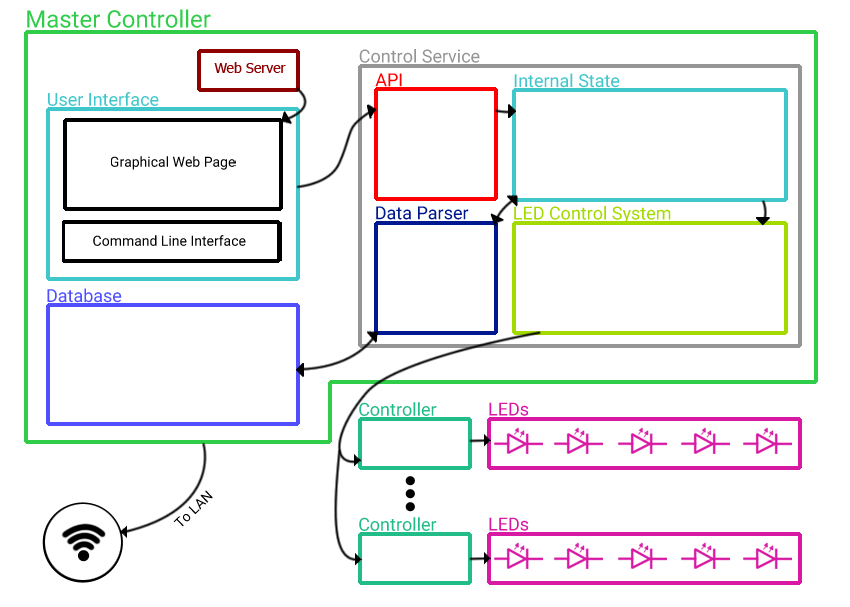
\includegraphics[width=\linewidth]{systemDiagrams/systemdiag.png}
				\caption{The PlanteR-GB system including interface and control systems}
				\label{fig:systemDiagram}
			\end{figure}
		\end{center}

		\subsection{Hardware}
			\subsubsection{Overview}
			\noindent The hardware controls the LEDs as well as run software. This software
			consists of controlling the LEDs, checking time, and other additional
			features such as a hosting a local web page. Because of the robust needs of
			the software, two different controllers are used.

			\noindent Two controllers are used, a Teensy 3.2 for LED control, and a Raspberry Pi Zero W for timing
			and additional features.
			\subsubsection{Master Controller}
			\noindent The Raspberry Pi Zero W was chosen to be the master controller for its
			multitasking capabilities. Raspberry Pi Zero W uses a ARM11 processor
			running at 1GHz with 512MB of RAM. \cite{pizero} The Pi Zero W has built in wireless and
			Bluetooth chips, allowing access to a wireless network without the need
			of additional hardware. This cuts down on the cost of the build and
			simplifies the build.

			\noindent The Raspberry Pi Zero W's ability to host a local web page while also
			keeping time makes this perfect to use as the master controller. The
			master controller is in charge of web hosting for iteration 6,
			data storage, and system state control. The Pi Zero W sends data to the LED controller which in turn controls
			to the LEDs.
			\begin{center}
				\begin{figure}[H]
					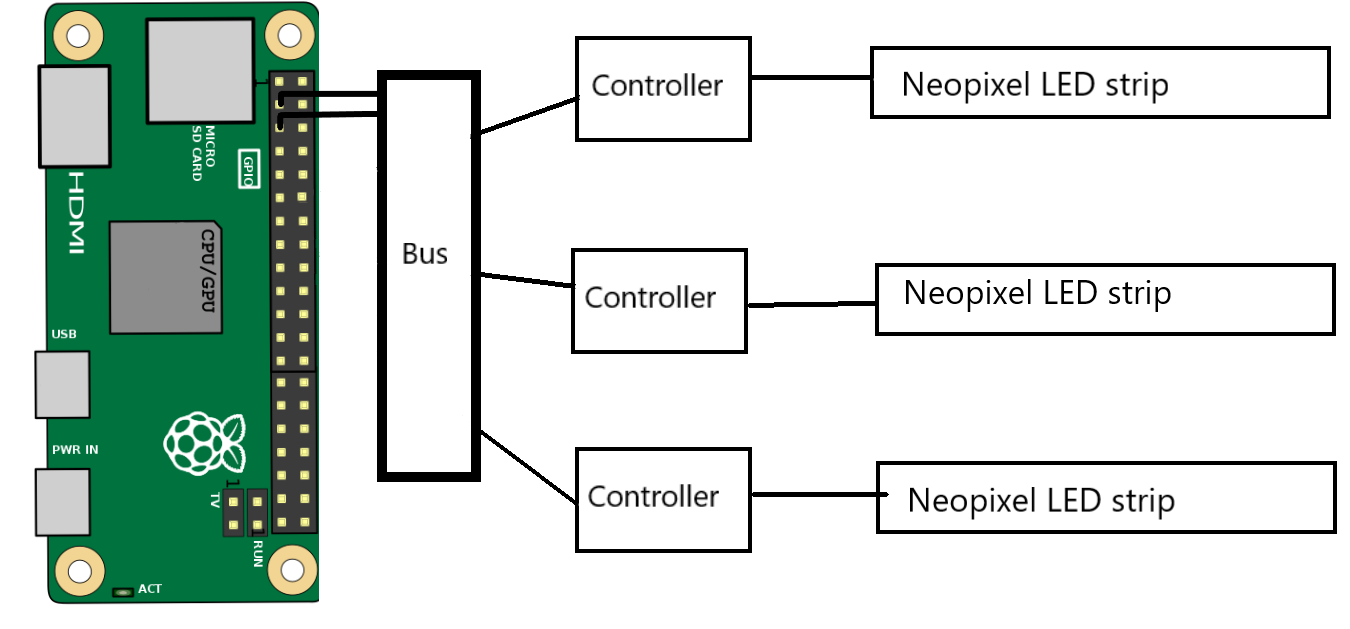
\includegraphics[width=\linewidth]{systemDiagrams/pischem.png}
					\caption{Raspberry Pi Zero W schematic}
					\label{fig:piSchematic}
				\end{figure}
			\end{center}
			\subsubsection{LED Controller(s)}
			\noindent The Teensy 3.2 was chosen for its ability to run Arduino and C programs.
			The size of the Teensy also makes this a great choice as reducing the
			total size of the build cuts down on the minimum size of each box.
			The Teensy 3.2 runs an updated Cortex-M4 with 64kB of RAM making this a
			better choice than the Teensy 2.0.\cite{atmel} The Teensy 3.2 can run Arduino code as well as the third party LED control library FastLED.

			\subsubsection{LED strips}
			\noindent The LEDs are the WS812 Neopixel LED strips by Adafruit. These LED
			strips are fairly thin, at 12.5mm wide with the included casing. The
			Neopixel LEDs are fully compatible with the FastLED library and are fully addressable.\cite{neo}

		\subsection{Control Service}
			\subsubsection{Overview}
			The control service is the bridge between the user interface and the LEDs.
			It has an API that serves as the entry point for all system changes, an internal state representation which is fed to the LED control system and also translated into persistent storage.
			The API obfuscates the communication between the client UI and the control service by providing a set of routes through which data can be sent.
			To make a data request or modification, the client sends data to the control service using one of the REST verbs (GET, POST, PUT, DELETE, etc).
			Using the REST protocol simplifies communication between client and server, but also allows new settings and parameters to quickly become accessible through the addition of new routes.

			\noindent \\The control service internal state is the primary representation of the configuration and settings of the system.
			This internal state is the focal point of the API, data storage, and LED control system.
			It is responsible for representing all data and committing it into persistent storage.
			When a client UI makes a change to a system parameter, the data is routed through the API and into the internal state.

			\noindent \\The data parser is responsible for translating the system state into persistent storage when changes are made.
			When the system starts, the data parser reads from persistent storage and rebuilds the internal state.
			A database with tables closely mirroring the internal state objects is the persistent end of the data parser.

			\subsubsection{API}
			%pistache.io is a good REST library for C++
			The API implements a REST protocol. REST is an architectural style and modern approach to web service communication. \cite{rest1}
			It provides a lightweight communication protocol between client and server, making it a popular building style for cloud-based APIs.
			The control service API consists of a series of routes, each relevant to a particular parameter or set of parameters.
			The internal state is updated when a client sends a request to the API.

			\noindent \\Here is an example of a series of REST requests which build a basic functioning system:
			\begin{lstlisting}[language=XML]
// Create an LED state with ID 3
PUT http://localhost:5324/ledstate/3
// Set the color of LED state 3 to red
POST http://localhost:5324/ledstate/3/color/ff0000
// Set the intensity of LED state 3 to 85%
POST http://localhost:5324/ledstate/3/intensity/85
// Set the power of LED state to on
POST http://localhost:5324/ledstate/3/power/on

// Add a new schedule with ID 4
PUT http://localhost:5324/schedule/4/
// LED state 3 triggers at 8:30am
POST http://localhost:5324/schedule/4/hour/0830/ledstate/3
// LED state 4 triggers at 2:00pm
POST http://localhost:5324/schedule/4/hour/1600/ledstate/4
// LED state 0 triggers at 9:00pm
POST http://localhost:5324/schedule/4/hour/2100/ledstate/0

// Add a new zone with ID 3
PUT http://localhost:5324/zone/3/
// Set the schedule used by zone 3 to schedule 4
POST http://localhost:5324/zone/3/schedule/4
// Assign LEDs 1 through 4 to zone 3
POST http://localhost:5324/zone/3/leds/1-4
// Assign LEDs 6 through 8 to zone 3
POST http://localhost:5324/zone/3/leds/6-8
// Assign LED 9 to zone 3
POST http://localhost:5324/zone/3/leds/9

// Get the current color of zone 3
GET http://localhost:5324/zone/3/color/

// Delete zone 3
DELETE http://localhost:5324/zone/3/
\end{lstlisting}

			\subsubsection{Internal State}
			The internal state of the system is represented by a series of objects closely mirroring their physical counterparts.
			An object is a template that can be instantiated into memory, and then manipulated.
			Using objects allows the system to represent its properties in a human readable way, as well as easily translate them into persistent storage and LED controller data.

			\noindent \\In this system, the smallest unit of measurement is the LED. The properties assigned to groups of LEDs defines the behavior of the system as a whole.
			A strip may have any number of individually controllable LEDs, attached to an LED controller.
			The Controller contains all information needed for the Control Service to locate and communicate with a physical LED controller.
			The Zone is the next highest unit of measurement, and represents a set of relationships between LEDs and a shared schedule of behavior.
			The LEDs within a zone can come from any number of LED strips attached to any LED controllers in the system.
			A schedule contains a series of time stamps each of which point to an LED state.
			Color, intensity, and power (on/off) are the three properties of an LED. An LED state defines a single combination of these properties, and can be assigned to a Zone at a specific time.


			\noindent \\This diagram shows the internal state of the control service:

			\begin{center}
				\begin{figure}[H]
					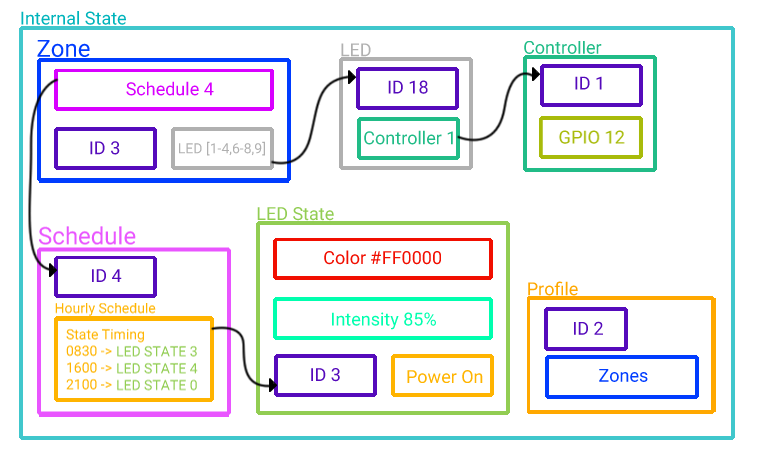
\includegraphics[width=\linewidth]{systemDiagrams/internalstate.png}
					\caption{The Internal state of the Control Service is the primary data representation, which is translated as necessary to persistent storage and LED control system.}
					\label{fig:internalStateDiagram}
				\end{figure}
			\end{center}

			\subsubsection{Data Parser}
			The data parser serves as a translator between internal state and persistent storage.
			Data flows from the Control Service API, into the internal state, and then finally to the Data Parser where the data is saved.
			The data parser has a series of functions which take internal state objects as parameters, and generate queries that are ran against the database.
			In addition to saving data, the data parser has functions that query the database and return internal state objects.
			Lastly, the data parser is responsible for any conversion routines necessary should the data format be changed significantly between iterations.


		\subsection{Data Design}
			\subsubsection{Overview}
			% Probably SQLite, because MySQL is a memory hog
			The persistent data storage is done with a database.
			The Data Parser in the Control Service translates the internal state into a series of SQL commands to INSERT, UPDATE, or DELETE from the data tables.
			A database is used because of its ability to update, delete, or read a single piece of information without requiring the entire data structure to be read into memory.
			When changes are made to the way data is structured in the internal state, the database can be restructured and updated with a short script.

			\noindent \\These are the tables that exist within the database:
			\begin{center}
				\begin{figure}[H]
					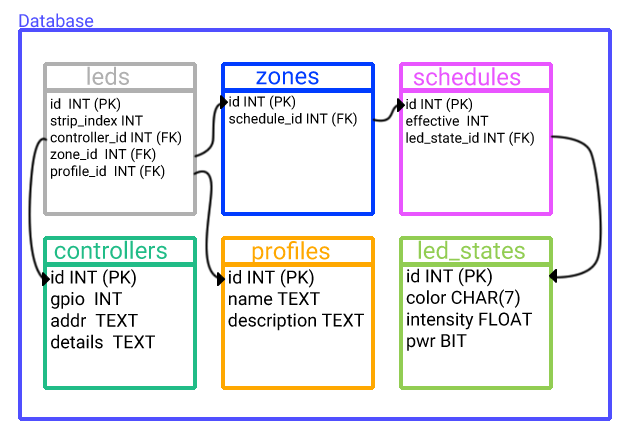
\includegraphics[width=\linewidth]{systemDiagrams/database.png}
					\caption{Schema Diagram of the database tables}
					\label{fig:databaseDiagram}
				\end{figure}
			\end{center}

			\subsubsection{Data Description}
			In the database, LEDs are stored with an ID, zone, profile, and controller. Zones store the schedule that all LEDs within it follow.
			Schedules store LED states and the time that each becomes active. LED states store color, intensity, and the power state.
			Lastly, profiles store a name and description, but each LED itself stores the Zone it belongs to per Profile.

			\noindent \\The tables below contain example data that represents how a real system might look.

			\subsubsection{LEDs table}
				\begin{tabular}{ |c|c|c|c|c| }
					\hline
					id (INT) & strip\_index (INT) & controller\_id (INT) & zone\_id (INT) & profile\_id (INT) \\
					\hline
					1 & 1 & 1 & 1 & 1 \\
					2 & 2 & 1 & 2 & 1 \\
					3 & 3 & 1 & 1 & 1 \\
					4 & 4 & 1 & 2 & 1 \\
					5 & 1 & 2 & 1 & 1 \\
					6 & 2 & 2 & 2 & 1 \\
					7 & 3 & 2 & 3 & 1 \\
					8 & 4 & 2 & 3 & 1 \\
					\hline
				\end{tabular}

			\subsubsection{LED States table}
				\begin{tabular}{ |c|c|c|c| }
					\hline
					id (INT) & color (CHAR(7)) & intensity (FLOAT) & pwr (BIT)\\
					\hline
					1 & 000000 & 0 & 0 \\
					2 & FF0000 & 85 & 1 \\
					3 & 00FF00 & 60 & 1 \\
					4 & 0000FF & 60 & 1 \\
					\hline
				\end{tabular}

			\subsubsection{Zones table}
				\begin{tabular}{ |c|c| }
					\hline
					id (INT) & schedule\_id (INT) \\
					\hline
					1 & 1 \\
					2 & 1 \\
					3 & 2 \\
					\hline
				\end{tabular}

			\subsubsection{Schedules table}
				\begin{tabular}{ |c|c|c| }
					\hline
					id (INT) & effective (INT) & led\_state\_id (INT) \\
					\hline
					1 & 800 & 2 \\
					1 & 1800 & 1 \\
					2 & 430 & 3 \\
					2 & 934 & 4 \\
					2 & 2200 & 1 \\
					\hline
				\end{tabular}

			\subsubsection{Profiles table}
				\begin{tabular}{ |c|c|c| }
					\hline
					id (INT) & name (TEXT) & description (TEXT) \\
					\hline
					1 & ``Default'' & ``The default schedule that happens every day'' \\
					2 & ``Holiday'' & ``Lights flash green and red for 30 minutes in the morning, then return to normal'' \\
					2 & ``Vacation'' & ``Lights come on earlier in the morning and turn off later'' \\
					\hline
				\end{tabular}

			\subsubsection{Controllers table}
				\begin{tabular}{ |c|c|c|c| }
					\hline
					id (INT) & gpio (INT) & addr (TEXT) & details (TEXT) \\
					\hline
					1 & 26 & ``NULL'' & ``NULL'' \\
					2 & 17 & ``NULL'' & ``NULL'' \\
					3 & 0 & ``DF:48:16:A3:44:2B'' & ``protocol:3'' \\
					\hline
				\end{tabular}


		\subsection{LED Control System}
			\subsubsection{Overview}
				\noindent LED control System is be handled by two different controllers. The master controller handles human input, while the LED controller handles the LED input such as color, intensity, and power state.
				This allows a single controller to handle communication to the LEDs, as the
				LEDs are clock based and can be interfered by other processes. \cite{fastLED}
				\subsubsection{LED Controller Communication}
				\noindent Communication between the master controller and LED controller is done via a serial link.
				A serial link capable of sending user data through the Pi, to the Teensy, and out to the LED strip can be formed by connecting pins eight and ten of the Pi Zero TX and RX respectively, to the Teensy pins zero and one.
				The Pi Zero translates what is given from the user to serial, and then send it to the Teensy. The Teensy then communicates the received serial data to the LEDs via the FastLED library.
				\subsubsection{LED Controller Software}
				\noindent FastLED is the library chosen that is used on the LED controller.
				As the name implies, the library is a fast LED library created for Arduino projects.
				Initialization code would look like this:

			\begin{lstlisting}
#define NUM_LEDS 10 // number of LEDs on the strip. use only number of LED's on the strip
#define DATA_PIN 6 // pin used for data signal

void setup(){
	FastLED.addLeds<WS812>(leds, NUM_LEDS)
}

void loop(){
	leds[0] =  CRGB::Red; //sets the first LED to red
	fastLED.show(); // library call to display
	delay(30); //refresh every 30 cycles
}

		\end{lstlisting}

			\section{Human Interface Design}
			        \subsection{Overview of User Interface}
			        They way humans interface with a program is an important part of any program.
			        For this project there are two iterations of the human interface. The
			        first being thgouh the command line. The second is a web interface.
			        \subsection{Command Line Interface}
			            \subsubsection{Interface Overview}
			            The command line interface asks questions of the user about how they
			            would like to configure the settings. There are 5 options to
			            choose from in the main menu. Those options are: Bed Options, Zoning Options,
			            Scheduling Options, Profile Options and the final option is to apply changes.
			            Each Option as sub options to configure that section. For example in the
			            scheduling section there is a prompt to edit a schedule or to add a schedule.
			            If edit schedule is chosen the system prompts the user to choose which
			            schedule to modify and then specific settings such as start time, color, and brightness are chosen.
			            Once all the options are filled in the system return to the page where you can apply the changes.
			            \subsubsection{Command Line Mockup}
			            \begin{center}
			                \begin{figure}[H]
			                    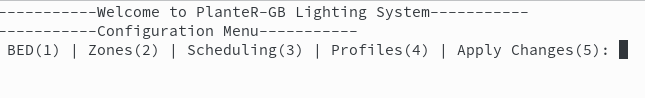
\includegraphics[width=\linewidth]{comand_line_interface/Selection_006.png}
			                    \caption{Start of Command Line Interface}
			                    \label{fig:Start of Command Line Interface}
			                \end{figure}

			                \begin{figure}[H]
			                    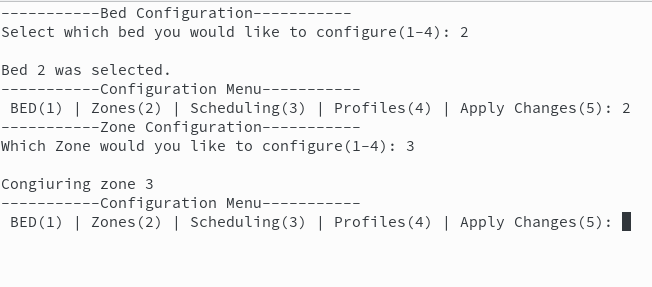
\includegraphics[width=\linewidth]{comand_line_interface/Selection_003.png}
			                    \caption{Bed and Zone Selection Menu}
			                    \label{fig:Bed and Zone Selection Menu}
			                \end{figure}

			            \begin{figure}[H]
			                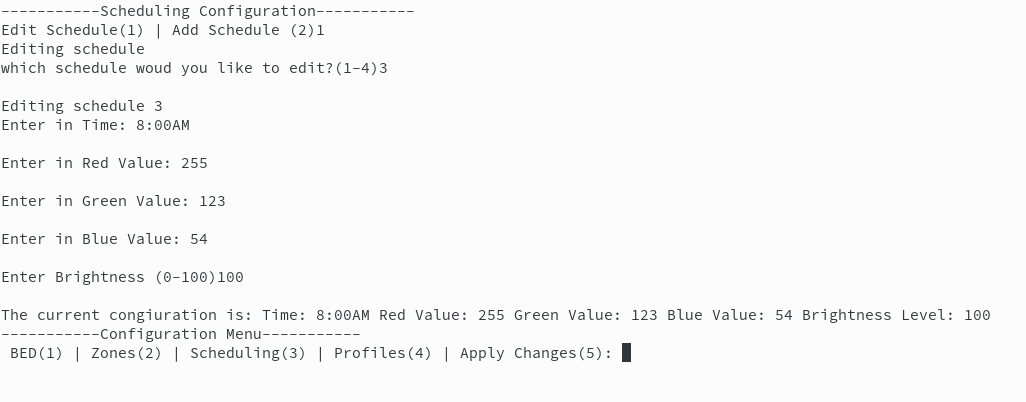
\includegraphics[width=\linewidth]{comand_line_interface/Selection_004.png}
			                \caption{Scheduling Configuration Menu}
			                \label{fig:Scheduling Configuration Menu}
			            \end{figure}

			            \begin{figure}[H]
			                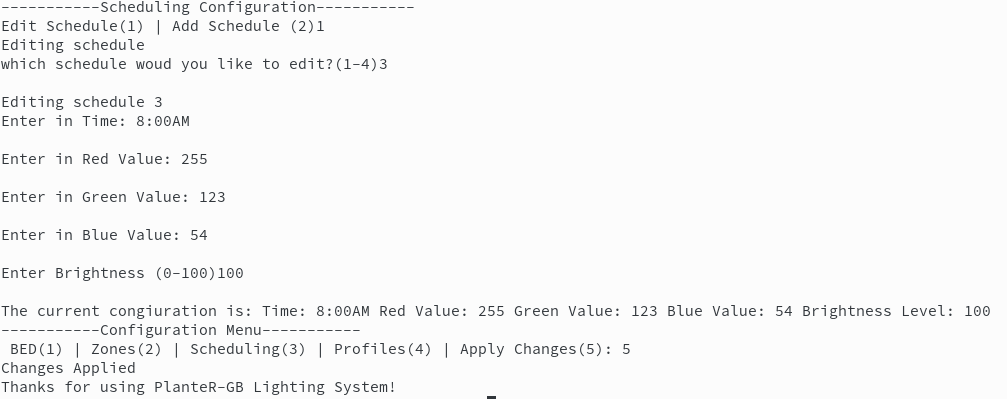
\includegraphics[width=\linewidth]{comand_line_interface/Selection_005.png}
			                \caption{End of Command Line Interface}
			                \label{fig:End of Command Line Interface}
			            \end{figure}
			        \end{center}

			        \subsection{Web Interface}
			            \subsubsection{Interface Overview}
			            The web interface consists of four pages to configure the settings of
			            the lighting system. The pages are the home page where the bed that the user
			            wishes to modify is selected. The Zoning page where the user can select
			            the zones the user would like to set on the LED strips. A Scheduling page
			            to set up schedules for when to turn on and off, what color and how bright.
			            The last page is the profile page where a user can create and change profiles.
			            The currently selected bed and profile appear in the top right corner.
			            Below, each page is discussed in greater detail and a mockup of each page
			            is displayed.
			            \subsubsection{Home Page}
			            The home page of the web interface prompts the user to select which
			            bed they would like to modify. If the user only has one bed hooked up there
			            is only one option. The chosen bed appears in the top right corner under Currently
			            Selected.
			            \subsubsection{Home Page Mockup}
			            \begin{center}
			                \begin{figure}[H]
			                    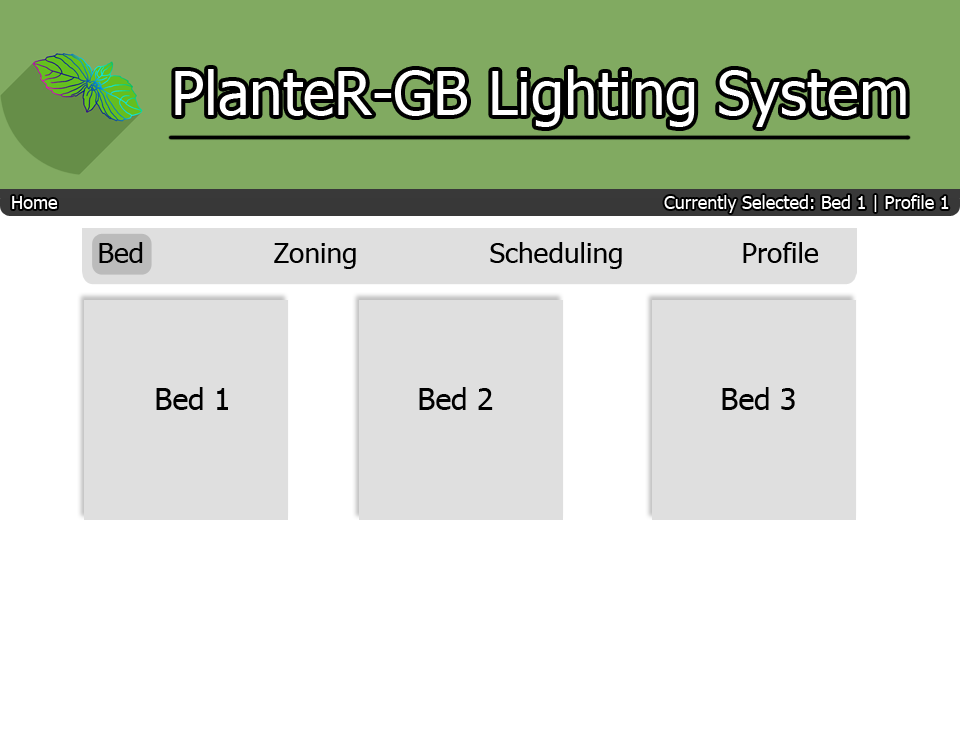
\includegraphics[width=\linewidth]{web_design/BedPage.png}
			                    \caption{Home Web Page}
			                    \label{fig:Home Page}
			                \end{figure}
			            \end{center}
			            \subsubsection{Zones Page}
			            The zoning section of the web page is where the user sets zones on
			            the LEDs. All LED strips that are on the selected bed are shown, and the user can assign each LED to a zone by click on it.
									The number of zones can be increased by clicking the "Add Zone" button.
									They appear below with the color that is assigned to that zone. You can then select
			            which zone you would like to add LEDs too by clicking the drop down menu "Select Zone".
			            When you add an LED to a zone a box with that color appears around it
			            and grow as more LEDs are added to the zone.
			            \subsubsection{Zoning Page Mockup}
			            \begin{center}
			                \begin{figure}[H]
			                    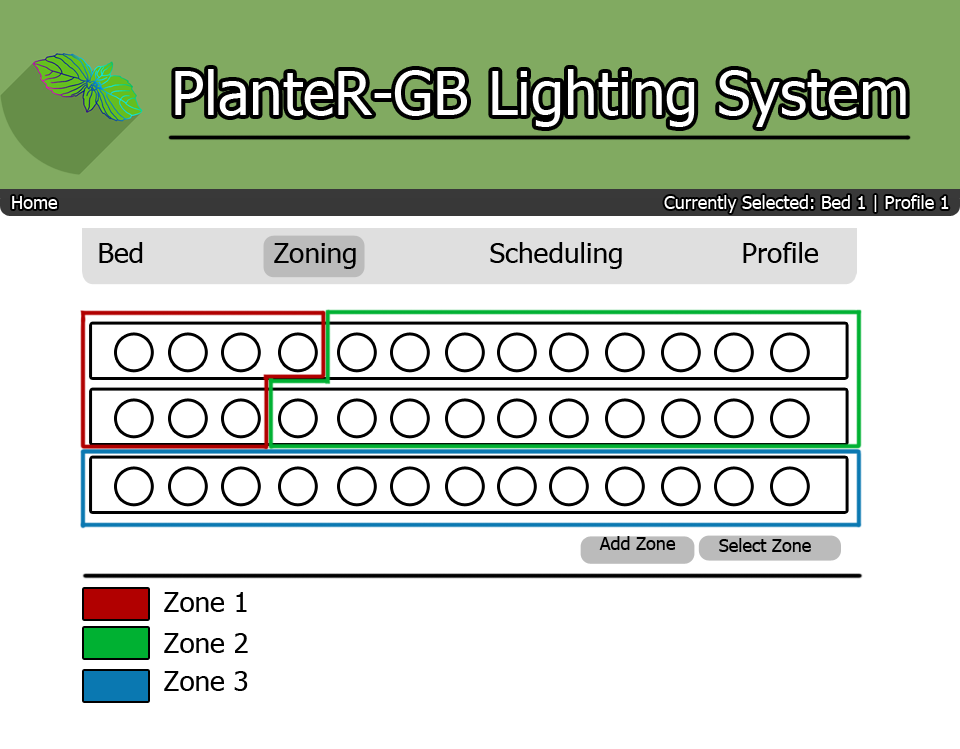
\includegraphics[width=\linewidth]{web_design/ZoningPage.png}
			                    \caption{Zoning Web Page}
			                    \label{fig:Zoning Page}
			                \end{figure}
			            \end{center}
			            \subsubsection{Schedule Page}
			            The schedule page is where the main part of the configuration is done.
			            This is where you would select what time color and brightness of the LEDs.
			            You can have different schedules for different zones. You can add new schedule
			            by clicking the "Add Schedule" button and a new schedule is added to the
			            list.
			            \subsubsection{Schedule Page Mockup}
			            \begin{center}
			                \begin{figure}[H]
			                    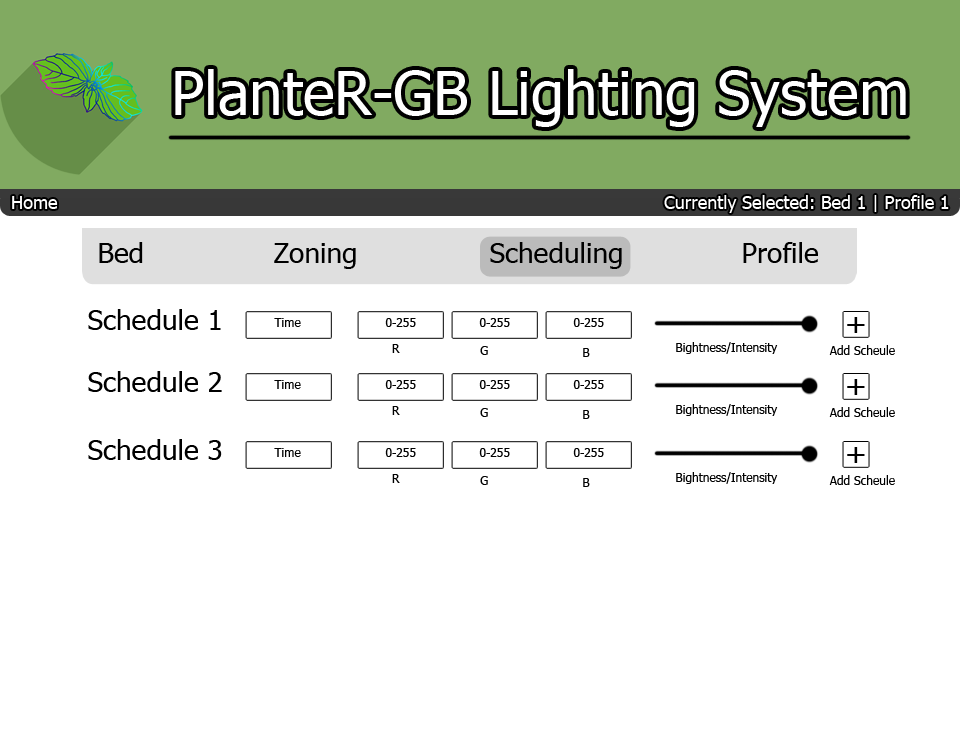
\includegraphics[width=\linewidth]{web_design/SchedulingPage.png}
			                    \caption{Scheduling Web Page Mockup}
			                    \label{fig:Schedule Page}
			                \end{figure}
			            \end{center}
			            \subsubsection{Profile Page}
			            The profile page is where you can switch or create new profiles. The profile
			            that is currently selected is in the top right of the screen under the "Currently
			            Selected" section.
			            \subsubsection{Profile Page Mockup}
			            \begin{center}
			                \begin{figure}[H]
			                    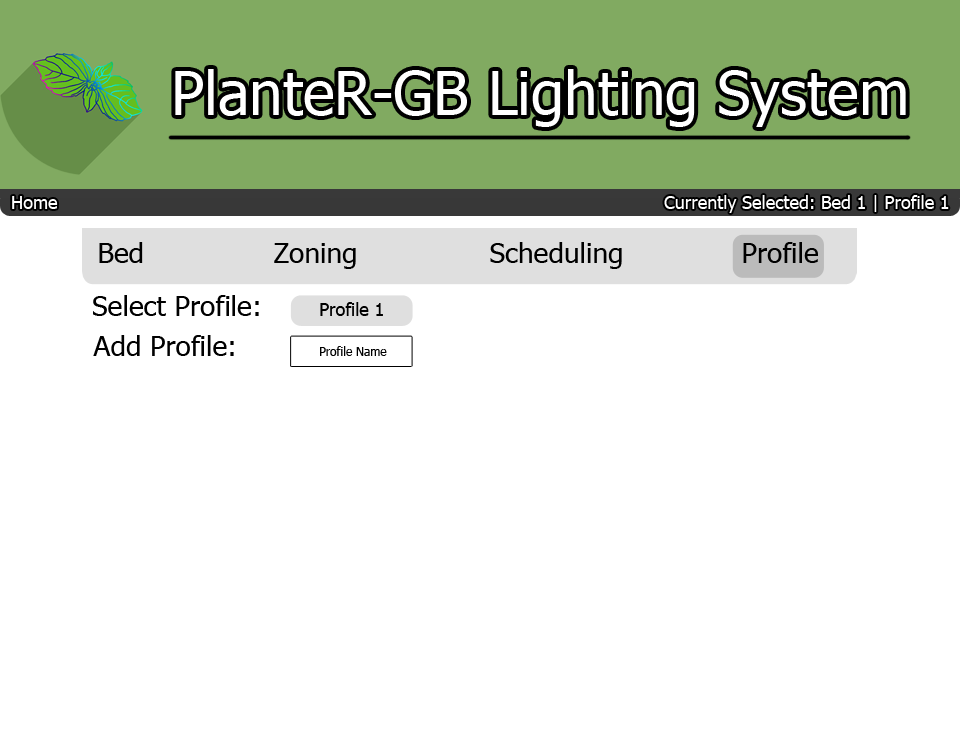
\includegraphics[width=\linewidth]{web_design/ProfilePage.png}
			                    \caption{Profile Web Page Mockup}
			                    \label{fig:Profile Page}
			                \end{figure}
			            \end{center}


	% Scheduling
	\section{Project Timeline}
		\subsection{Overview}
		Looking at the general timing of each of the described implementations, and given roughly 13 weeks, plus or minus a week, each iteration of the project
		should be given about two weeks of time. This allow plenty of time to be spent on each iteration. If an iteration takes less time than expected, this
		allows work to start on the next iteration early. The more iterations that are completed early, the more the iterations contained in the
		\textbf{Additional Features - v2.0} and \textbf{Stretch Goals - v3.0} can also potentially be completed.

		\subsection{Iteration 0}
		Iteration 0 accomplishes rough connectivity between the RGB strips and the microcontroller system. This means the Master controller can provide input
		to the LED controllers to manipulate trivial options like color and brightness. This iteration is only expected to take a maximum of 2 weeks, and may
		take closer to the end of those two weeks. This is the initial "get the ball rolling" iteration. It is expected there may be some complications
		getting used to the code environment, and getting the hardware up and running.

		\subsection{Iteration 1}
		Iteration 1 builds on Iteration 1 by making the LED controller look for values and configurations on the Master controller. These are scheduled
		statically. This is more of a testing iteration to see what the capabilities of communication are between the two controllers. This time will likely decrease.
		However, it still leaves time should any new issues arise in the details of the design.

		\subsection{Iteration 2}
		Iteration 2's largest feature is the scripting of the basic LED controls. A user may run a text based script to insert values into the control
		service. This updates the LEDs quickly, but may not be user friendly. This may also be a shortened iteration interval. The passing of
		data is completed, and a script is now taking over for manual updates. This script may also be the base for which future command line interfaces to the
		LEDs are made.

		\subsection{Iteration 3}
		This iteration sees the first basic functionality of scheduling the LED timings. Currently, the requirements state the iteration includes daily or
		weekly changes, but could also include hourly start timings for a specific LED state. Seeing as this iteration requires the implementation of a clock,
		and potentially multiple schedules running, this iteration could take the entire two weeks of the interval.

		\subsection{Iteration 4}
		Adding the largest functionality yet, Iteration 4 includes the implementation of LED zoning. Each zone has its own state and schedule. This iteration
		should almost certainly take the entire two week interval. This is due to the increased coding of the internal state housed by the master controller, which
		keeps a complete "image" of all zones, their specific LEDs, and schedules.

		\subsection{Iteration 5}
		Further building upon the previous iteration, Iteration 5 increases the amount of LEDs that can be driven, and the amount of control zones. This provides
		more precise control, and more options for future customization. This iteration is not expected to take the full two allotted weeks. Spending less time at
		this stage gives wiggle	room to the final iteration.

		\subsection{Iteration 6}
		Of the 7 iterations, Iteration 6 provides the largest boost of usability with a full fledged web interface. This web page, or set of pages, can provide
		the end	user the graphical representation of the current planter bed and all its LEDs. It also gives them full control of color, brightness, zoning,
		and scheduling, all within a few clicks. This iteration should take the remaining time left. If it turns out that it is completed early, the next set of
		iterations can be attempted.


	\section{Technology Review}
		\subsection{Austin Hodgin}
		% Document body
\section{Web Server Options}
	\subsection{Overview and Criteria}
	For our user interface we will be developing a web application to interface
	with the control system. There three criteria that are needed for our web
	server for this project. The first is that the server will need to run on
	our controller that we chose. The second being that the server will need to
	be reliable on starting up and maintaining the server over long stretches of
	time. The third being memory and processor efficient. The controllers that
	we will be using will have limited memory and we will have other tasks
	running on the same controller so having a server that uses less memory and
	still maintains the features that we require is important.
	\subsection{Potential Choices }
	There is three different web servers that are under consideration. The first
	being Apache. Apache is a HTTP server project produced by Apache Software. The
	second web server is Lighttpd. Lighttpd is a web server that is an open source
	project. The third option is Niginx web service produced by NGINX Software.
	Below we will discuss each of these options and if they meet the criteria
	that is required for this project.
	\subsection{Apache Web Server}
	Apache web server that is developed by Apache Software. It is a widely used
	web server. Reviewing their about page \cite{Apache}, they talk about
	building a stable and advanced web server that is robust, featureful, and
	free for anyone to use. This benefits us since we will not have to pay to use
	this server. Apache web server is also a process based server, this means
	that each connection gets its own thread on the CPU. This allows for if there
	is an error on one connection it does not bring down the whole server. This
	makes the server more reliable and stable. Apache is also for flexible configuration
	.htaccess files. It also comes standard on most Linux servers. Since it is
	one of the more popular options for web server it also has a lot of documentation.
	\\\\
	\textbf{Advantages}:
	\begin{itemize}
		\item \textbf{Stable}: Apache is a very stable web server which his helped
		with how it handles requests in multiple threads.

		\item \textbf{Documentation}: With Apache being one of the most widely used
		web servers there is a lot of documentation. When problems occur this will
		be beneficial.
	\end{itemize}

	\noindent\textbf{Disadvantages}:
	\begin{itemize}
		\item \textbf{Resources}: The drawback of having head request
		handled by a single thread on the CPU is that it requires more resources
		compared to the alternatives.
	\end{itemize}

	\subsection{Lighttpd Web Server}
	Lighttpd web server is a lightweight web server that is designed to be secure,
	fast, flexible and is optimized for high-performance. From their website \cite{Lighttpd}
	they state that they use non-blocking I/O event loop for running each single
	process that comes to the server. They talk about how the have a low memory
	footprint. Lighttpd is also an asynchronous server compared to Apache which is
	a synchronous server. Below are the advantages and disadvantages of using
	Lighttpd Web Server for our project.
	\\\\
	\textbf{Advantages}:
	\begin{itemize}
		\item \textbf{Fast and Lightweight}: With the server running on one thread
		and assigning working threads as well as the system uses non-blocking I/O
		event looping the server uses very little resources.
	\end{itemize}
	\noindent\textbf{Disadvantages}:
	\begin{itemize}
		\item \textbf{Not as Stable}: With the server running a single master thread
		and assigning worker threads, if something goes wrong with a connection casuing
		that thread to crash you lose the whole server.
		\item \textbf{Documentation}: With Lighttpd not as widely used, there
		is less documentation surrounding it. This can make solving problems down the
		road more difficult.
	\end{itemize}
	\subsection{Nginx Web server}
	Nginx is an open source web server developed by Nginx software. It is another
	asynchronous lightweight HTTP server. It differs from apache by that it has
	one master process to server requests. It then delegates tasks to worker
	proccess. This allows it to be very fast and efficient when serving static
	web pages. \cite{Nginx}. Below are the advantages and disadvantages
	of using Nginx web server for our project.
	\\\\
	\textbf{Advantages}:
	\begin{itemize}
		\item \textbf{Fast and Lightweight}:With the server running on one thread
		and assigning working threads as well as the system uses non-blocking I/O
		event looping the server uses very little resources.
		\item \textbf{Documentation}: Nginx is more widely so there is more documentation.
		This will allow us to more quickly solve problems when they occur.
	\end{itemize}
	\noindent\textbf{Disadvantages}:
	\begin{itemize}
		\item \textbf{Not As Stable}: With the server running a single master thread
		and assigning worker threads, if something goes wrong with a connection casuing
		that thread to crash you lose the whole server.
	\end{itemize}
	\subsection{Discussion}
	Apache, Lighttpd, Nginx, they all handle serving web pages and processing
	request slightly differently. Apache for example uses a processes based approach.
	Meaning that each request gets its own thread on the CPU, this does require
	some overhead when it comes to resource. This is in contrast to both Lighttpd
	and Nginx web servers which are asynchronous servers are mainly event-driven
	and run on a single process and split into worker tasks from there to complete
	tasks. This makes them a little faster and requires less total resources to run.
	There is a problem with running a single master process if there is a problem
	with the connection it could bring the whole server down which would not happen to an Apache server since each
	connection is in its own thread. All three technologies meet the criteria for r
	reliability, efficiency, and controller compatibility, but each has its own
	advantage
	\subsection{Conclusion}
	Looking at all three options, chosen to go with the Apache web server.
	This web service will only server web pages to a limited number of clients.
	One of the main criteria that we were worried about was that
	it would be stable once we had it working. Apache being one of the most stable
	web servers due to it using a process based server if a problem occurs with
	the connections then it won’t bring down the whole system. With that it meets
	all of our criteria for our project.
\newpage
\section{Mobile Options}
	\subsection{Overview and Criteria}
	As mobile computing becomes more and more popular it is important to take
	that into consideration when designing products today. With mobile becoming
	more important in today's world we would like to add a mobile option to interface
	with our system. When choosing which option we would like to go with when
	incorporating mobile we have to look at three key criteria. The first being
	that it works on multiple mobile platforms, Android, and IOS. The second being
	that we would like it to be consistent with how the user interacts with the
	product.
	\subsection{Potential Choices}
	When looking at mobile options there are three main options to look at. The
	first being building a native mobile application for each platform. The second
	being building a mobile friendly web interface.The final one being building
	a dedicated mobile site which will be served to the user if requested from
	a mobile device.
	\subsection{Native Mobile Application}
	Building a native app for mobile  Building a native mobile
	app has several advantages and disadvantages when it comes to working with
	products.
	\\\\
	\textbf{Advantages}:
	\begin{itemize}
		\item \textbf{Full Mobile Friendly}: This is designed and implemented with
		mobile in mind. Making it a more friendly mobile environment.
		\item \textbf{Quick Load Times}: With the app fully contained on the mobile
		it does not have pull a web page from a server.
	\end{itemize}
	\noindent\textbf{Disadvantages}:
	\begin{itemize}
		\item \textbf{Developing and Maintaining Multiple Platforms}: With designing
		and creating a native mobile app you have to create it on two different platforms.
		This can be time consuming.
	\end{itemize}
	\subsection{Build Mobile Friendly Website}
	Wth building a mobile friendly website we would develop the site with mobile
	in mind. Building a mobile friendly website has several advantages and disadvantages
	when working with products. Below are listed the advantages and disadvantages
	for building a mobile friendly website.
	\textbf{Advantages}:
	\begin{itemize}
		\item \textbf{Consistent With Desktop Content}: This would allow the desktop
		and mobile environments to feel consistent and not make users learn two
		different interfaces
		\item \textbf{Less To Maintain}: Only once site needs to be built making
		maintaining the site easier.
	\end{itemize}
	\textbf{Disadvantages}:
	\begin{itemize}
		\item \textbf{General Usability}: Changing settings or checking the same
		information might be more difficult on a mobile platform due to how they go
		through the pages.
		\item \textbf{Slower Loading Times}: With the amount of information pushed
			back and forth between the device and could be slower due to it going over
			3g or 4g speeds.
	\end{itemize}
	\subsection{Build Mobile Dedicated Site}
	Building a dedicated mobile app would be creating the site again but more
	mobile friendly and delivering that to mobile devices instead of the desktop
	site. Below are the advantages and disadvantages of creating a mobile dedicated site.
	\textbf{Advantages}:
	\begin{itemize}
		\item \textbf{Mobile Focused}: With building a mobile dedicated site it allows
		you to make it more mobile friendly.
		\item \textbf{Consistent Style}: It allows for you to tweak the style of the
		main site to allow for it to be more mobile friendly but still keep its look
		and feel.
	\end{itemize}
	\textbf{Disadvantages}:
	\begin{itemize}
		\item \textbf{Increased Maintains Time/Cost}: With having two sites to maintain,
		you will have to put more time and energy creating and maintaining it.
		\item \textbf{Slower Service}: Since the server has to check what type of
		device that is requesting the page it takes some processing time.
	\end{itemize}
	\subsection{Discussion}
	Looking at all three options they all have advantages and disadvantages. For
	our project we are looking at a few key criteria and those are that it has to
	work on multiple platforms and that it needs to be consistent with the desktop
	environment. All three can easily be made to be consistent with the desktop
	environment. With building native application for mobile that would require
	applications developed for both Android and IOS. This is time consuming and
	difficult to maintain as a change in one would require a change in the other.
	This is in contrast to the other two options, where both of them will work on any device
	given that it has a browser. Looking at the other two options they both have very
	similar advantages and disadvantages. The main disadvantage to building a dedicated
	mobile site is that you will have to build and maintain two sites which compared to
	building a mobile friendly website where you just have to maintain one site.
	They both meet both criteria we have for our mobile options and are both strong
	options.
	\subsection{Conclusion}
	Between the three options, building a native mobile application, building a
	mobile dedicated site and building a mobile friendly site we choose to go with
	building a mobile friendly site. With keeping mobile devices in mind from the
	beginning of the web interface it makes it easier to develop and maintain over
	time. This also cuts down on development time over all as we only need to
	create one web site.
\section{Moisture Sensors}
	\subsection{Overview and Criteria}
	We would like to be able to add moisture sensors
	to the enclosure to monitor the moisture of the soil the plants are in to
	get an idea of when you should water your plants. To do this we have several
	criteria that we have to look at. The first being that it must be able to
	interact with our chosen microcontroller. The second being that it must
	read the moisture of the soil.
	\subsection{Potential Choices }
	There are three different choices that we could go with. The first is going
	with an Octopus soil moisture sensor from Elecfreaks \cite[pg 2] {Octopus_soil_sensor},
	We could design and custom print our own moisture sensors or we could go with
	a SparkFun Soil Moisture Sensor from SparkFun \cite[pg 2] {SparkFun_Soil_Moisture_Sensor}.
	\subsection{Octopus Soil Moisture Sensor}
	Octopus soil moisture sensor is a moisture sensor that can be purchased through
	Elecfreaks. This sensor is a lot like other moisture sensors in shape and how
	it connects to a micro controller. The way this moisture sensor is unique is
	that it can connect to the sensor modules. This can connect to any arduino
	based microcontroller.
	\\\\
	\textbf{Advantages}:
	\begin{itemize}
		\item \textbf{Time Investment}: With the sensors already built the only time
		need is to configure and install the sensors.
		\item \textbf{Cost}: For the first initial prototypes it is cheaper to use
		these.
	\end{itemize}
	\noindent\textbf{Disadvantages}:
	\begin{itemize}
		\item \textbf{Not Customizable}: We are not able to design the shape or features
		it monitors.
	\end{itemize}
	\subsection{Design and Print Own Sensors}
	One option would be to design our own sensor using a program like Eagle and
	have it printed and sent to use. The advantage to this is that we can make the
	sensor exactly how want it in the shape that would fit in our enclosure. This
	would also be ideal if we need a bunch of them. The disadvantage for this would
	that we would have to spend time designing it and then have to wait for them
	to print. This would only be ideal if we were going through to a production
	unit.
	\\\\
	\textbf{Advantages}:
	\begin{itemize}
		\item \textbf{Customizable}: With designing and building our own sensors
		we can add only the features that are needed for the project.
		\item \textbf{Cost}: This is the cheapest options when buying large quantities.
	\end{itemize}
	\noindent\textbf{Disadvantages}:
	\begin{itemize}
		\item \textbf{Large Investment}: To design and have the sensors made would
		take a large investment of time and money. In the long run it would be advantageous
		to do this if this goes to production.
	\end{itemize}
	\subsection{SparkFun Soil Moisture Sensor}
	SparkFun soil moisture sensor  be purchased through Sparkfun. It can be used
	with any arduino microcontroller. This allows us to be able monitor the soil
	moisture. The SparkFun soil moisture sensor is a lot like many other sensors
	in design and how it interfaces with microcontrollers.
	\\\\
	\textbf{Advantages}:
	\begin{itemize}
		\item \textbf{Time Investment}: With the sensors already built the onlly time
		need is to configure and install the sensors.
	\end{itemize}
	\noindent\textbf{Disadvantages}:
	\begin{itemize}
		\item \textbf{Not Customizable}: We are not able to design the shape or features
		it monitors.
		\item \textbf{Cost}: These are more expensive than other sensors on the market.
	\end{itemize}
	\subsection{Discussion}
	Moisture sensors are simple sensors so most of them are similar in shape,
	size and how they read in moisture. For this reason it is possible to design
	our own and get it the shape and size that we would like. The disadvantage of this
	is that we would have to design it and then have them printed and they are
	not guaranteed to work. This is why the other two options were chosen. The
	Octopus Soil Moisture Sensor and the Sparkfun Soil Moisture Sensor are very similar
	The Octopus soil moisture sensor has the ability to connect to other sensors.
	This is a nice feature if we would like to add any other sensors. The SparkFun
	Soil moisture sensor doesn't have any special feature other than reading in
	the moisture level. Though it is more expensive than the Octopus moisture sensor.
	\subsection{Conclusion}
	Looking at all the options it seems like the Octopus soil moisture sensor is
	the option we will be going with. Designing and having it printed would be
	time consuming and expensive up front. The SparkFun soil moisture sensor is
	has all the features that we need but is more expensive than the Octopus soil.
	The added cost of this sensor makes Octopus soil moisture sensor the sensor
	we will be using for our project.


		\subsection{Travis Hodgin}
		% Document body
\section{Microcontroller}
	\subsection{Overview and Criteria}
	The microcontroller will run parts or all of our software. With this in mind,
	we need to find a controller that fits within certain criteria. The
	controller must
	\begin{itemize}
		\item Controller is reprogramable
		\item Controller contains I/O pins
	\end{itemize}
	The controller must be reprogramable as to allow the user to change files;
	This also facilitates testing. The I/O pins will allow the LED strips to
	interface with the controller, as well as allow additional features to be
	added.

	\vspace{5mm}
	\noindent Following these criteria, we have a few additional features that would be
	benifical. These include:
	\begin{itemize}
		\item Controller allows multiple applications to run simultaneously
		\item Controller allows connection via a wireless network
		\item Controller is capable of hosting a web page
	\end{itemize}
	Allowing the controller to run multiple applications will facilitate
	multiple features to run on a single controller; For example the controller
	will run the LED interface, as well as hosting a web page. Allowing
	connection via a wireless network will help with additional features on a
	single controller.
	\subsection{Potential Choices}
	During our research we have found three commonly used microcontrollers that
	fit our criteria. The first is the Teensy 3.2. The second is the Arduino Uno,
	and the third is the Raspberry Pi Zero W. These three were chosen for their
	ease of use, price, and documentation.
	\subsection{Teensy 3.2}
	The Teensy 3.2 is a commonly used microntroller for small scale LED projects,
	using a cortex-m4 ARM processor running at 72MHz \cite[Pg 7]{K20}. Storage consists
	of 256KB of flash memory that will contain the Arduino or C flashed to it.
	The Teensy has 34 I/O pins, and is powered by 5V supplied by a micro USB
	cable.

	\vspace{5mm}
	\noindent The Teensy 3.2 is a fairly small board, being only 1.4 inches long
	by 0.7 inches wide, which is great for projects where space is limited. The
	Teensy 3.2 is priced at \$20.

	\vspace{5mm}
	\noindent Advantages of the Teensy 3.2:
	\begin{itemize}
		\item Small form factor
		\item Runs Arduino and C programs
		\item Compatible with many LED libraries
	\end{itemize}
	Disadvantages of the Teensy 3.2:
	\begin{itemize}
		\item Not robust enough for much more than the LEDs
		\item Documentation is lacking with regards to LEDs
	\end{itemize}
	\subsection{Arduino Uno}

	\vspace{5mm}
	\noindent The Arduino Uno is a popluar microcontroller for many small electronics
	projects. The Uno contains an ATmega328 controller running at 20 million
	instructions per second (MIPS) at 20MHz with 32KB of flash
	memory\cite[Pg 7]{atmel}. Containing 14 digital I/O pins of which 6
	can be used for PWM outputs, and six analog inputs \cite[Pg 7]{arduino}.
	The Uno uses an input voltage of 5v off a barel jack. The Uno has a large community with
	a lot of documentation.

	\vspace{5mm}
	\noindent The Arduino Uno is 2.7 inches by 2.1 inches making it more ideal for
	projects where size isnt a limiting factor.

	\vspace{5mm}
	Advantages of the Arduino Uno:
	\begin{itemize}
		\item Compatible with many LED libraries
		\item Addon shields allow for further features to be added
		\item Interfacing with the LEDs is easiest with this device
		\item Documentation is fantastic
	\end{itemize}
	Disadvantages of the Arduino Uno:
	\begin{itemize}
		\item Shields sold seperatly
		\item Not robust enough to run more than LEDs and sensors
		\item Wireless connections require more hardware.
	\end{itemize}
	\subsection{Raspberry pi Zero W}

	\vspace{5mm}
	\noindent The Raspberry Pi Zero W is more of a microcomputer than a microcontroller.
	It is capable of running a full linux operating system and
	contains an ARM processory at 1GHz with 512MB of RAM making this the most
	powerful option we looked at. This Pi uses 40 GPIO pins for
	external interface, uses a micro SD card for storage, and supports digital
	video out via a mini HDMI\cite[Pg 7]{pizero}.

	\vspace{5mm}
	\noindent Additionally, the Pi Zero W contains a wireless and bluetooth chip built in.
	The Pi Zero W is another small controller being 2.5 inch by 1.2 inch
	making this controller another great choice for smaller projects.
	Raspberry Pi Zero W is priced at \$10, with a huge community and plenty of documentation.

	\vspace{5mm}
	\noindent While the Raspberry Pi can run many RGB LEDs, specific models use internal
	clock timings to time the LED signals. This makes running these on the Pi,
	which uses a multi-tasking linux operating system, a pain.

	\vspace{5mm}
	\noindent Advantages of the Raspberry Pi Zero W:
	\begin{itemize}
		\item Can host local web pages
		\item Can run a light linux operating system
		\item Great documentation
	\end{itemize}
	Disadvantages of the Raspberry Pi Zero W:
	\begin{itemize}
		\item Multitasking operating system make clock based LEDs a pain to
		work with.
	\end{itemize}

	\subsection{Discussion}
	\noindent Each of these controllers meet our
	requirements. The Teensy, being our least powerful device, is a great choice
	for small LED projects. It appears the Teensy will not be able to handle
	both setting the LEDs and changing the time the LEDs will turn on and off
	at the same time. This makes the Teensy a great option for only a part of
	the project.

	\vspace{5mm}
	\noindent The Arduino Uno, being our second most powerful device on the
	list, is capable of handling both setting the LEDs and changing the time
	the LEDs will turn on and off. This makes it a great option for this
	project. Since it is an Arduino, we are limited to two coding languages;
	Arduino, and C. The only way for the Uno to connect to a wireless network,
	is by using an external shield or USB wireless adapter. This means we will
	need additional hardware to connect to any network.


	\vspace{5mm}
	\noindent The Raspberry Pi Zero W is the most powerful controller option on
	this list. This gives us more options in terms of additional
	features. With its great support, amount of GPIO pins, and ability to run
	several applications at the same time, this is would be a great option for
	a sort of "master" running our some of our additional features such as a
	local web page, and moisture sensors, while another controller can handle
	the LED controls.

	\subsection{Conclusion}
	\noindent Given our criteria, and our additional features, we have decided
	to use the Raspberry Pi Zero W and a Teensy 3.2. Because of the power of the
	Pi Zero W, the ability to run a full linux operating system, price, size,
	and number of GPIO pins, this controller fits everything we need and more.
	The LED libraries make using the Teensy as the LED driver much more
	attractive.LED Libraries will be discussed in another section. The Pi Zero
	W's ability to host web pages, and connect to wireless networks with no a
	dditional hardware, we can achieve more of our additional features.

\section{LEDs}
	\subsection{Overview and Criteria}
	\noindent The LEDs are the centeral point of this project. As such, we need
	to pick a type that suits our needs. Our criteria are:
	\begin{itemize}
		\item The LEDs must be RGB
		\item The LEDs strips must be modular
	\end{itemize}
	\noindent The LEDs we choose have to be RGB, that is the point of this
	project. With modular LEDs, we will be able to create any size kit we want,
	depending on how many LEDs we want to use.
	\subsection{Potential Choices}
	\noindent We have three great choices for LEDs. The first is the Adafruit
	WS2812 Neopixel LED strip. The second is the DOTSTAR APA102 LED strip.
	Lastly we have the WS2801 diffused LED strand. Each of these fits all of
	our criteria.
	\subsection{Neopixel WS2812}
	\noindent The WS2812 Neopixel LEDs from Adafruit is popular for many LED
	projects. These LEDs are digitally addressable, meaning we can set each LED
	color individualy; Each LED has a shift-registers, chained throughout the
	strip which allows us to shorten the strip, or add more to the end
	\cite[Pg 7]{neo}. Once you set the color, you can disconnect the strip from
	the controller, and as long as its still being powered, it will remain
	thanks to the build in PWM into each LED-chip. Powering the LEDs comes
	from solder pads on the side of each LED that will provide 5V and up to 2A,
	ground, and a data line.


	\vspace{5mm}
	\noindent The Neopixel WS2812 LEDs come with 60 LEDs across a meter for \$24.99.

	\vspace{5mm}
	\noindent Advantages of the Neopixel WS2812:
	\begin{itemize}
		\item Documentation is great
		\item Digitally addressable
		\item Modular
		\item Many libraries
	\end{itemize}
	Disadvantages of the Neopixel WS2812:
	\begin{itemize}
		\item Clock controlled
	\end{itemize}
	\subsection{DOTSTAR APA102}
	\noindent The DOTSTR APA102 are an alternative to adafruits Neopixel LEDs. Instead
	of working on a single data pin, these work on a 2-wire SPI, meaning data
	can traverse the strip much faster than the Neopixel PWM system. These do
	not require timing meaning clock cycles will not affect these
	\cite[Pg2]{dotstar}. These contain 30 LEDs per meter with 24-bit color,
	8 bits for each red, green, and blue. Like the Neopixel, each LED acts Like
	a shift register, which means we can, if not hardware limited, control an
	infinite number of LEDs. The full meter costs \$19.95.

	\vspace{5mm}
	\noindent Advantages of the Dotstar APA102:
	\begin{itemize}
		\item SPI allows data to travel faster down the LED strip.
	\end{itemize}
	Disadvantages of the Dotstar APA102:
	\begin{itemize}
		\item Less LED per meter than Neopixel
		\item SPI can be hard to set up
		\item Documentation is lacking
	\end{itemize}
	\subsection{WS2801 Diffused LED Strand}
	\noindent The WS2801 LED strand runs similarly to the Neopixel LEDS as they
	are clock based. Instead of a strip, they are in a strand of weatherproof
	"dots" that fit through a 12mm hole\cite[Pg 7]{strand}. These are diffused
	LEDs meaning the light is spread more evenly, reducing hard edges and
	shadows. Like the other two options, these are 24-bit colors. Similarly to
	the Neopixel's thes are PWM driven and must be clocked by the controller.

	\vspace{5mm}
	\noindent These only come in strands of 25, making these not easily modular without
	modifications. They are run off of 5V at up to 2A, just like the previous
	choices and are priced at \$39.95.

	\vspace{5mm}
	\noindent Advantages of the WS2801 Diffused LED Strands:
	\begin{itemize}
		\item Diffused lighting helps reduce hard shadows
		\item Dot based LED gives more options for hiding wiring
		\item Many libraries
	\end{itemize}
	Disadvantages of the WS2801 Diffused LED Strands:
	\begin{itemize}
		\item Not easily modular
		\item clock controlled
		\item Forced to use 25 pixels
	\end{itemize}
	\subsection{Discussion}
	The WS2812 and the WS2801 use the same clock based control, making the only
	difference is the style of LED. Both the WS2812 and the DOTSTAR LEDs are
	strips of flat LEDs, with the Dotstar being about \$5 cheaper.

	\vspace{5mm}
	\noindent The DOTSTAR uses an SPI connection from the making it an interesting choice.
	The major complaint is the lack documentation.
	\subsection{Conclusion}
	\noindent Because of the documentation, the libraries supported, and size,
	we have chosen to go with the WS812 Neopixel LEDs. These are the LEDs we
	have seen for many different projects, has great documentation from both
	Adafruit, and users, is supported by many libraries, and can be split up
	into smaller strips if needed, makes this our best choice.


\section{LED Libraries}
	\subsection{Overview and Criteria}
	\noindent LED libraries are what the microcontroller uses to interface with
	the LEDs. We need to pick a library that fits with our microcontroller, and
	LED choice. It is important to note that there exists libraries to run
	clock based LEDs on the raspberry pi using hardware PWM. These, however
	are created by other users, and are not updated often. Our
	criteria are:
	\begin{itemize}
		\item Library must work with either the Raspberry Pi, or Arduino Uno
		\item Library must work with the WS2812 Neopixel LEDs
	\end{itemize}
	\noindent We need to be sure the library we want to use is compatible with
	the controller we are using, otherwise the whole project will not work.
	Similarly, we need to make sure the library can work for the LEDs of our
	choice.
	\subsection{Potential Choices}
	\noindent For libraries, we have several choices. The first is fastLED. The
	second is the Adafruits Neopixel library, and the third choice is to build
	our own library. Each of these options will fit our criteria.
	\subsection{FastLED}
	\noindent FastLED is an arduino based library created to make programming
	LEDs faster and easier. This library has support for both SPI, and 3-wire
	chipsets\cite[Pg 7]{fastLED}. Many projects found using the Neopixel LEDs
	used this library.

	\vspace{5mm}
	\noindent This library is written in C++ and can be used in for anything
	that can run Arduino, such as the Arduino Uno and Teensy 3.2. Supporting
	both SPI and 3-wire chipsets allow for many different types of LEDs to
	interface, however it cannont be used on multi-tasking devices such as the
	raspberry pi. This is mostly due to the LEDs supported have a problem with
	clock timing, with the exception of LEDs such as the APA102.

	\vspace{5mm}
	\noindent Advantages to FastLED:
	\begin{itemize}
		\item Supports many different LED structures
		\item Great documentation
	\end{itemize}
	Disadvantages to FastLED:
	\begin{itemize}
		\item limited to running on Arduino
	\end{itemize}
	\subsection{Adafruit Library}
	\noindent The Adafruit Neopixel Library is specifically designed for their Neopixel
	LEDs. This library is written in C++ and is made for use for Arduino
	projects. That means this can be run on anything that can run Arduino such
	as the Arduino Uno and the Teensy 3.2. Adafruit has an article discussing
	the use of the library\cite[Pg 7]{neolib}.


	\vspace{5mm}
	\noindent Past this, the library has little in the way of documentation. The article
	discusses basic use, but doesn't go into much past their test script. This
	will lead to more time spent digging into the code base. In our research we
	have found many different projects using this library.

	\vspace{5mm}
	\noindent Advantages of the Adafruit Neopixel Library:
	\begin{itemize}
		\item Built specifically for Neopixel
		\item Built for use on Arduino devices
	\end{itemize}
	Disadvantages of the Adafruit Library:
	\begin{itemize}
		\item Can only use Neopixel LEDs
		\item Documentation is a little lacking
	\end{itemize}
	\subsection{Build our Own}
	\noindent Building our own library will reduce a lot of our problems of other
	libraries. We can code specifically for the LED and controller we want.
	This reduces the amount of added code the controller will use. Additionally,
	we will have better knowledge of how to write the project, as we are the
	ones who wrote it.

	\vspace{5mm}
	\noindent The major problem that comes with building our own LED library is time.
	Havig to write our own library will require extensive resarch, writing, and
	testing time that can detract from our original project.
	\subsection{Discussion}
	\noindent FastLED is a very popular LED library used in many projects we found
	during our research. With its broad LED support, and great documentation,
	it is an appealing option. The Neopixel library, while only made for use on
	the Neopixel LEDs, isn't bloated by the addition of these other LED types.
	Building our own library would allow us to intergrate only features we need
	for the specific LED type we are using. This however, will require more
	time for us to complete.
	\subsection{Conclusion}
	\noindent Because of the documentation and LED support, we have decided to use
	FastLED as our LED library. FastLED has great support, and allows many LED
	types for future expansion if needed.

		\subsection{Zach Lerew}
			% Document body
		%Purpose of tech, derived from tech, example usage, projects that use.
		%Critical thinking, research, comparison to other tech
	\section{Control Service API}
		\subsection{Overview and Criteria}
		The control service is the bridge between the user interface and the LEDs.
		The API (application programming interface) will serve as the entry point for all changes made to the system.
		The method with which the UI and the control service communicate is obfuscated from the user, but is an important factor in the speed and reliability of the system.
		The control service interface needs to be versatile enough to support the rapid addition of new features, and simple enough that it does not become a bottleneck in the system.

		\subsubsection{REST}
		REST stands for \textbf{Re}presentational \textbf{S}tate \textbf{T}ransfer.
		It is an architectural style and modern approach to web service communication. \cite[ch.5]{rest1}
		REST provides a lightweight communication protocol between client and server,
		making it a popular building style for cloud-based APIs.
		It is used commonly all over the web, and by companies like Amazon, Microsoft, and Google. \cite{rest2}
		The architecture provides a limited set of actions (verbs) which accompany each request and determine how the data is processed: GET, POST, PUT, and DELETE.
		Flexibility is provided by assigning resources (nouns) to a specific URL.
		REST applications typically send data over HTTP, which can be parsed by existing web technologies, meaning it can be displayed or analyzed in a web page easily.

		\noindent \\In the context of this system, a request to a REST driven Control Service could look like this:
		\begin{lstlisting}[language=XML]
POST http://localhost:5324/api/update/zone/
Host: localhost
Content-Type: text/xml; charset=utf-8
Content-Length: 123
<?xml version="1.0" encoding="utf-8"?>
<Zone>
  <ID>3</ID>
  <Color>RED</Color>
  <Intensity>40</Intensity>
  <PwrState>On</PwrState>
</Zone>
		\end{lstlisting}


		\noindent \\The control flow of the Control Service with a REST API may look like this:

		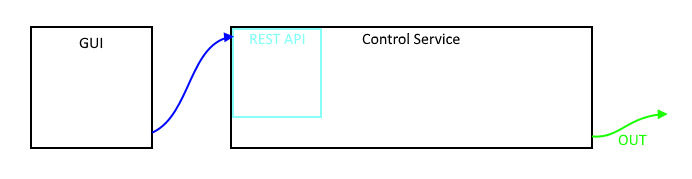
\includegraphics[width=\linewidth]{RESTDiag.png}

		\noindent \\Advantages of using REST architecture:
		\begin{itemize}
			\item Adding new data manipulation routes is simple and fast, simply bind a route (\textit{/api/update/schedule/}) to a function (\textit{void UpdateSchedule(request)})
			\item Control Service and interface are separated and do not need to understand each other's inner structure to transfer data
			\item Control Service can assume the role of the \textit{server} in the client-server model by responding to client requests, removing the need for a nodeJS web server to take in requests
			\item Control Service can respond to local network requests with no extra effort, allowing the GUI to be hosted on a different networked device (distributed systems)
		\end{itemize}

		\noindent \\Disadvantages of using a REST architecture:
		\begin{itemize}
			\item Language support is mostly ubiquitous, but some library implementations may be better than others
			\item HTTP may have some minor overhead
		\end{itemize}

		%GUI (Makes changes and sends cross-origin input to REST API) ->
		%Control service (Listens for CRUD requests, ex:localhost:8324/api/edit/zone/1/color/red) ->
		%Control service (Updates internal system state and writes to config file for persistence) ->
		%Control service (Gets submit request, )
		%Control service - Pull changes from config file, and incorporate changes into driving language file ->
		%Upon _localhost:8324/api/submit_ - Control service - Recompile driving language file, do something with the hex

		\subsubsection{File manipulation}
		File manipulation is a method of communication where the web server and Control Service communicate through the direct modification of a shared configuration file.
		This system works by having a standard configuration file structure which is known by both the web server and control service.
		System settings are changed in the client interface and posted to the web server, which opens and modifies the configuration file it shares with the control service.
		The Control Service monitors the configuration file for changes, and reloads its internal state when changes are detected.
		There are several options for configuration files, such as XML, JSON, or YAML. \cite{config1}
		Using this option would leverage the Unix file system for data transfer between web server and control service.

		\noindent \\In this system, the control flow for a file manipulation interface may look like this:

		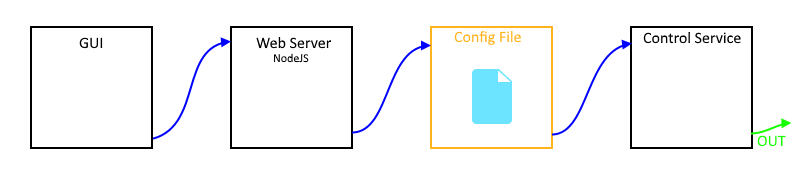
\includegraphics[width=\linewidth]{FileManipDiag.png}

		\noindent \\Advantages of using file manipulation:
		\begin{itemize}
			\item Persistent storage would come automatically
		\end{itemize}

		\noindent \\Disadvantages of using file manipulation:
		\begin{itemize}
			\item File I/O is very time consuming, and requires the entire file to be read each time a change is made
			\item The web server and control service both need to read and write to the configuration file, requiring the maintenance of two parsing functions in different languages to be maintained
			\item File manipulation must be synchronous - the system cannot read and write to the file at the same time
		\end{itemize}

		%GUI - Front end client makes changes ->
		%GUI - Javascript back end of some sort that takes client requests and reads (parses) config file, writes changes
		%Control service -> Reads changes to config file (parses), update internal state ->
		%Control service -> Applies changes through GPIO or recompile HEX

		\subsubsection{Socket IPC}
		Socket IPC (inter-process communication) is a method of communication where the web server and Control Service communicate through a socket connection.
		Socket communication works by establishing a communication link between a client and the server, which remains open for the duration of the transaction. \cite{socket1}
		Once data is transferred, the socket is closed. Sockets can communicate between devices on a local network, or between processes on a single device.


		\noindent \\In this system, the control flow for a socket IPC interface may look like this:

		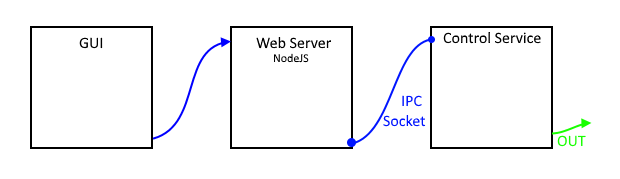
\includegraphics[width=\linewidth]{IPCDiag.png}

		\noindent \\Advantages of using sockets:
		\begin{itemize}
			\item Natively supported by any language considered for the system
			\item Efficient and fast communication
		\end{itemize}

		\noindent \\Disadvantages of using sockets:
		\begin{itemize}
			\item Bare-bones, all communication details and protocols would have to be custom written, re-inventing the HTTP wheel
			\item Would require web server to open dedicated socket connection to Control Service for every client connection
		\end{itemize}


		\subsection{Discussion}
		All three of these technologies will allow clients to communicate with the Control Service, but not all of them would meet the criteria for versatility and simplicity.
		Features will be rapidly added to the system, meaning the time spent modifying existing communication code should be minimized if possible, as it will be done often.
		Using a REST API eliminates the need for a dedicated web server by moving the client communication logic into the Control Service. It also allows changes to be made easily and rapidly, but some additional overhead is accrued in exchange for reduced development complexity.
		Using file manipulation eliminates the need for a persistent data storage system by modifying the saved disk data directly, at the expense of a speed loss.
		File manipulation also requires two code bases to be maintained for reading and writing the configuration file (web server and control service).
		Using sockets for communication is fast and efficient, but difficult to correctly implement, as very little is given automatically.
		Sockets only provide a channel for data to flow, so data transfer protocols and communication standards must be manually implemented.

		\subsection{Conclusion}
		Due to the rapid change schedule employed by this system, the ability to easily modify how data is transferred between client and server is an important factor when choosing an API technology.
		A REST API provides the most versatility and is the easiest to use out of the three options, making it the preferred choice for the Control Service API.


	\section{Control Service data storage}
		\subsection{Overview and Criteria}
		The data storage system is a crucial component of the Control Service.
		It will allow data to persist between system reboots, and serves as a backup allowing data to be copied to a new system.
		When system settings are modified, the changes travel through the Control Service, and end by modifying the LEDs.
		While setting changes are within the Control Service, they will be saved to the file system to allow user settings to persist in the frequent event of a system power loss.
		The most important aspect of data storage for this system should be maintainability.
		The constant iteration of this system will require the data's structure to be changed frequently, and possibly dramatically.
		The second most important aspect is accessibility. Reading and writing data using the system should be a simple process.
	  The third aspect is speed. The data will be stored on a device with limited processing capabilities. Saving or loading data should not be a bottleneck to system performance.

		\subsubsection{Serialization}
		Supported by most high level object oriented languages, serialization is a process by which an object is converted into a stream of bytes and then stored in a database, file, a different section of memory, or a networked device. \cite{serialization1}
		The reverse operation is called deserialization, which allows a stored file to be directly converted back into an object in memory.
		The process of serialization can be used to send object data directly from one system to another, without requiring a manual conversion routine to be written.

		\noindent \\In this system, the control flow for object serialization may look like this:

		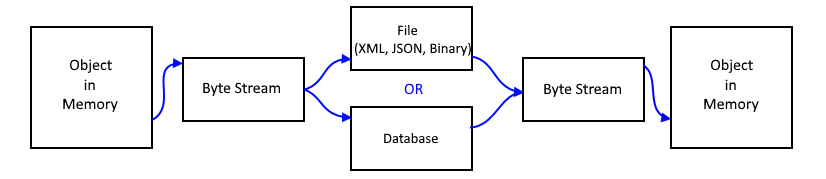
\includegraphics[width=\linewidth]{serializationDiag.png}

		\noindent \\Advantages of using serialization:
		\begin{itemize}
			\item Supported by any object oriented language considered for the project
			\item Massively simplifies saving and loading
			\item Objects can be converted directly to human readable XML, JSON, or straight to binary data
		\end{itemize}

		\noindent \\Disadvantages of using serialization:
		\begin{itemize}
			\item Loading old data after object changes have been made requires a manual conversion routine
			\item Data may take up slightly more disk space than storing raw data
		\end{itemize}


		\subsubsection{Database}
		Database are groups of highly organized data that can be easily created, retrieved, updated, and deleted. \cite{database1}
		Databases are organized into tables and rows, indexed to provide very fast and efficient data access.
		A database is typically a file or collection of files stored in a particular format that is probably not human readable.
		The data is accessed using a query language, of which there are many (SQLite, MySQL, T-SQL, SQLServer, etc).
		In typical usage, an SQL query is written and sent to an SQL service for processing and retrieval.
		The result is returned to the source that requested it.
		It is then processed row by row, where it is manually converted into a format usable by the system.

		\noindent \\In the context of this system, a database request may look like this:
		\begin{lstlisting}[language=SQL]
/* Insert new zone, ID 3, RED, 80% intensity, schedule 1 */
INSERT INTO ZONES (ID, COL, INTENS, SCHED_ID) VALUES (3, "FF0000", 0.8, 1);
/* Insert new zone, ID 4, GREEN, 40% intensity, schedule 2 */
INSERT INTO ZONES (ID, COL, INTENS, SCHED_ID) VALUES (4, "00FF00", 0.4, 2);

/* Get four columns from the zone with an id of 3 */
SELECT ID, COL, INTENS, SCHED_ID FROM ZONES WHERE ID = 3;

/* Change the color of the zone with an id of 4 to BLUE */
UPDATE ZONES SET COL = "0000FF" WHERE ID = 4;
\end{lstlisting}

		\noindent \\A loading routine that reads SQL data to produce internal objects may look like this:

	\begin{lstlisting}[language=JAVA]
Result result = SQL.executeQuery("SELECT * FROM ZONES");
while (result.next()) {
	int ID = result.getInt("ID");
	int Color = result.getInt("COL");
	float Intensity = result.getFloat("INTENS");
	Schedule WeekSchedule = Schedules.get(result.getInt("SCHED_ID"));

	Zone z = new Zone(ID, Color, Intensity, WeekSchedule);
	Zones.Add(z);
}
\end{lstlisting}

\noindent \\Advantages of using a database:
\begin{itemize}
	\item Very large amounts of data can be stored without difficulty or performance loss
	\item Storage, retrieval, and modification of data is simple and fast
	\item Data conversion can be done directly in SQL with not much difficulty
\end{itemize}

\noindent \\Disadvantages of using a database:
\begin{itemize}
	\item Separate query language required for data access
	\item Some SQL services are efficient for large amounts of data at the cost of overhead
\end{itemize}


		\subsubsection{Translation to markup}
		Internal object state can be converted into a markup configuration file and stored in plain text.
		There are several languages to choose from for markup (XML, JSON, Yaml) \cite{config1}
		A conversion function is written that takes an object and manually translates it into a format required by the chosen configuration language.
		Once the file is saved, it can be opened again and manually translated back into a memory object.

		\noindent \\In this system, the control flow for object translation to markup may look like this:

		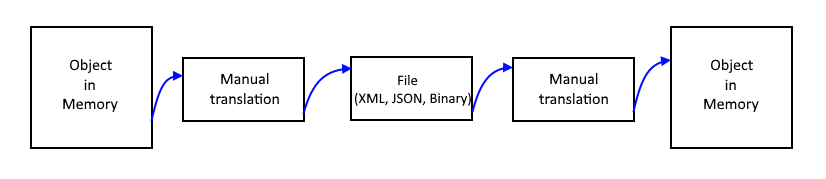
\includegraphics[width=\linewidth]{markupDiag.png}

		\noindent \\Advantages of using markup translation:
		\begin{itemize}
			\item Full control over data storage and conversion
		\end{itemize}

		\noindent \\Disadvantages of using markup translation:
		\begin{itemize}
			\item Manual translation functions (saving and loading) must be written and modified every time a change is made to any data structure
			\item Conversion of stored data from previous data format can be difficult and is required every time data changes
		\end{itemize}


		\subsection{Discussion}
		All three of these options solve the issue of persistent data storage, each has a different level of maintainability and speed.
		Serialization allows saving and loading to become trivial, nearly automatic.
		The downside is that every change to the way data is structured requires a manual translation function to be written and then thrown away.
		Using a database requires translation routines for saving and loading, but data conversion becomes simple and can be done entirely within the database.
		Serialization is easy to set up, but difficult to maintain. Databases are difficult to set up, but easy to maintain. Markup translation is difficult to set up and maintain.

		\subsection{Conclusion}
		Due to the constant iteration of the system, converting data will be a frequent and important part of the development cycle.
		That is why a database is the recommended method for the persistent storage of data.

		\section{Control Service internal state}
			\subsection{Overview and Criteria}
			The internal state of the service could be described as its short term memory.
			Input is received and processed, output to the LEDs, and then stored using long term storage if necessary.
			The internal state lets the system (and the user) know what previous input was received, without performing a time consuming long term storage retrieval.
			The system can store the current data for all LEDs, user profile settings, schedules, and any other piece of relevant information.
			That information can then be easily translated into serial data for the LEDs, file data for persistent storage, and web data for GUI display.
			The rapid iteration cycle of this system means that settings and data will change frequently and possibly dramatically.
			The internal structure of the system state should be easily modified to allow these changes to happen with little resistance.


			\subsubsection{Objects and classes}
			Object oriented programming (OOP) is a paradigm loved by some, and hated by others.
			Objects are instances of a template (\textit{class}). More or less, a class is like an ice cube tray, and objects are the resulting ice-cubes.
			An object is made up of variables (\textit{members}) and functions (\textit{behavior}).
			Objects allow complex data relationships to be expressed in real-world terms, trading some performance or memory for a simpler conceptual understanding, and a shorter development time.
			One of the most useful aspects of OOP is inheritance. Objects can inherit properties from other objects.
			For example, a \textit{Tesla Model S} is an automobile with a max speed, wheels, seats, and propulsion. But it has some additional traits such as a battery pack and autonomous driving that are not shared by every automobile.

			\noindent \\In this system, using Objects to represent internal state may look like this:

			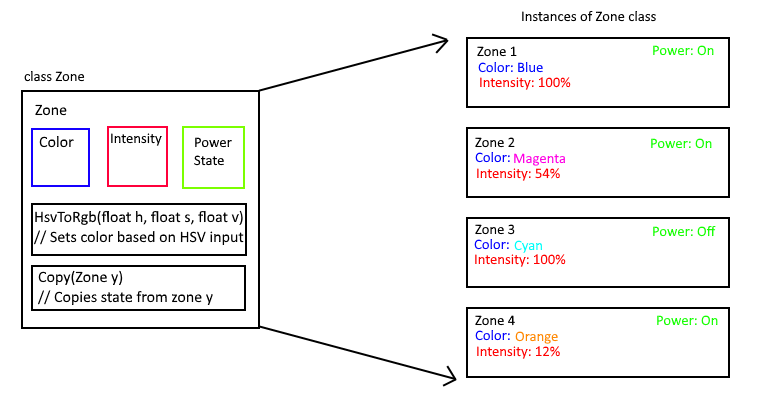
\includegraphics[width=\linewidth]{objectsDiag.png}

			\noindent \\Advantages of using objects:
			\begin{itemize}
				\item System structure and features are easily written in code, logic is organized and kept with related data
				\item Changes can be quickly and easily made
				\item Non-trivial data can be represented in an easy to understand way
			\end{itemize}

			\noindent \\Disadvantages of using objects:
			\begin{itemize}
				\item More memory is used when storing objects compared to raw integers and strings
			\end{itemize}


			\subsubsection{Structs and lists}
			Structs are a precursor to objects in many ways. They are a relic from the C programming language, but are still a useful method of representing data.
			Structures or \textit{structs} are collections of variables, usually stored consecutively in memory, which can be manipulated as singular objects, almost as if a struct is a named box in which like data can be stored.
			Structures are essentially objects without behavior. Data can be stored in a useful and organized manner, but all logic pertaining to that data must be performed in a different location.
			Lists would be used as a method of storing multiple structs of similar type (ex: zone, schedule, plant, userProfile).

			\noindent \\Advantages of using structs:
			\begin{itemize}
				\item Raw data can be organized into digestible chunks
				\item Effectively the same footprint as storing raw data
			\end{itemize}

			\noindent \\Disadvantages of using structs:
			\begin{itemize}
				\item Business logic and data kept in separate locations, making the bigger picture harder to see
			\end{itemize}


			\subsubsection{File system or database}
			This option forgoes the organization and structure provided by objects or structs, and places the system state directly into the persistent storage.
			Effectively, this method would involve the removal of short term memory in favor of immediately placing everything into long term memory.
			Using this method, the Control Service becomes an input-output machine whose purpose is to gather input from its API, read physical storage, and insert or modify existing data.
			When data is accessed using this method, the file storage is queried for the data, the data is processed, and the result is output to the LEDs.
			The Control Service would have no internal knowledge of the state of the system, instead relying on an I/O call when data is required.

			\noindent \\Advantages of using file system:
			\begin{itemize}
				\item Long term data storage is automatic
			\end{itemize}

			\noindent \\Disadvantages of using file system:
			\begin{itemize}
				\item I/O calls are expensive relative to in-memory manipulation of data
				\item Reading and writing cannot occur simultaneously, meaning the system cannot take user input while reading or writing data
				\item Processing data is difficult without a simple way to represent the data in memory
			\end{itemize}


			\subsection{Discussion}
			OOP is a modern programming paradigm used in almost all production systems where speed is not the most important factor.
			It is highly unusual for a production application to have no internal representation of data, simply because that method does not scale well for large systems.

			\subsection{Conclusion}
			Objects are a fantastic way to organize the structure of a system, as they allow the data and its relationships to be easily digested and modified.
			Logic and variables live side by side, allowing developers to practice separation of concerns.
			This project will be developed by a team of four developers, meaning that an understanding of the data structure is crucial for effective feature implementation.
			For that reason, the recommendation is to organize the system using Objects to store variable data and behavior.

		\subsection{Max Schmidt}
		% Document body
	%Purpose of tech, derived from tech, example usage, projects that use.
	%Critical thinking, research, comparison to other tech
\section{Network Interfaces}

	\subsection{Overview and Criteria}
	Version 2.0 of the RGB LED Planter Box begins the with the requirements that a web interface be developed for the controller.
	This web interface will hosted on the local controller (localhost), and only this controller will be accessible to it.
	This is true, only if there isn't a network infrastructure to allow this host to share its web interface to other devices.
	This network infrastructure must accomodate the web interface host, other clients wishing to interact with the LED array, and
	be as simple to setup and maintain as possible.  \\

	There are many different types of devices and protocols that allow devices to pass information to each other, and share resources.
	Some of these have become more prominent over time due to adaptation and adoption by the majority of industries worldwide.
	Most devices that need to share resources, do so within local limited bounds of an organization.
	Our web interface ideally should be accessible via a LAN or \textbf{L}ocal \textbf{A}rea \textbf{N}etwork.
	LANs connect computers, servers, printers, and embedded devices in a limited space such as a home, school, or office building. \cite{LAN1}
	However, the choice made should leave room to expand, allowing the web interface to be accessible outside the LAN, if the user is able to provide the necessary resources.

	\subsection{Potential Candidates}
	During our research our team has found three commonly used LAN implementations that fit our project's needs.
	The first is a star topology LAN Over Wire, the second is a star topology LAN over wireless radio, and finally a mesh topology LAN over wireless radio.

	\subsubsection{Star Topology LAN Over Wire}
	Most LANs are based on a star topology.  In this configuration, all end nodes, referred to as clients, are connected to a central hub, which is often a high speed router or switch.
	Each client is connected to the hub via a cable, which is almost always a twisted pair cable.\cite{LAN2}
	In this architecture, all clients are able to communicate to each other by passing their network traffic through the central router.

	\begin{center}
		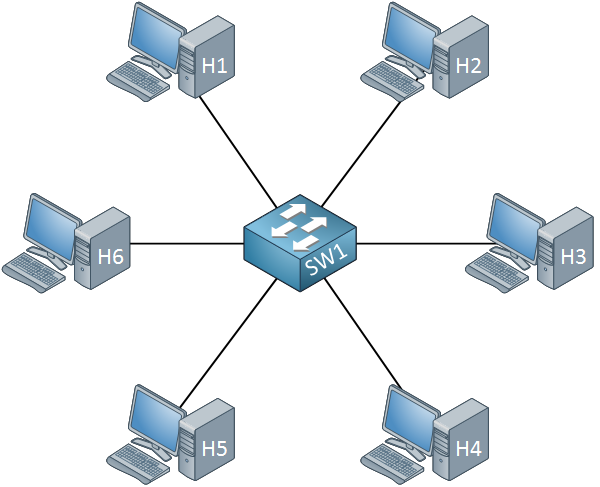
\includegraphics[scale=0.5]{switch-star-topology-hosts.png}
	\end{center} \cite{IMG1}

	\newpage % A better place to break and transition to new page

	\noindent \\ \textbf{Advantages} of using Wire Based Star Topology LANs:
	\begin{itemize}
		\item Traffic sent over wire is guaranteed to reach the destination node, provided the hardware is available.  Having a static physical medium to transfer data across means no data loss.
		\item Connecting new nodes to the network is seamless with IP protocols like DHCP (Dynamic Host Configuration Protocol).
		\item Traffic speed is not inhibited by environmental structure of surrounding area.  As long as the wire connects, one has a constant connection speed.
		\item A single client could fail, but others may continue to communicate on the network due to the architecture.
	\end{itemize}

	\noindent \\ \textbf{Disadvantages} of using Wire Based Star Topology LANs:
	\begin{itemize}
		\item The network infrastructure requires a decent amount of hardware.  Each client that wants to connect needs a wire.
		\item Since all traffic is mediated by a central hub:
		\begin{itemize}
			\item If the hub fails, no clients may communicate with each other or the web interface host.
			\item The hub could become a bottleneck for all network resources under heavy traffic.
		\end{itemize}
	\end{itemize}

	\subsubsection{Star Topology LAN Over Radio}
	This LAN type is nearly the exact same as the wired version, except that clients connect to a hub via wireless radio protocols rather than a cable.
	Standards like IEEE-802.11 allow devices to communicate over radio waves on specific frequencies to pass information to each other.\cite{LAN3}

	\noindent \\ \textbf{Advantages} of using Wireless Radio Based Star Topology LANs:
	\begin{itemize}
		\item Network infrastructure doesn't require much hardware.  Clients and hub need adapters to communicate via radio waves.
		\item Clients can move around freely, and aren't tied down by fixed length cables.  Cables can also physically get in the way.
	\end{itemize}

	\noindent \\ \textbf{Disadvantages} of using Wireless Radio Based Star Topology LANs:
	\begin{itemize}
		\item Wireless radios have to convert wireless signals into understandable frames, and could be slower than wired due to conversion
		\item Radio waves behave like light waves, in that physical objects like walls, can impede the transmission of data.  Data transmission is not guaranteed in every case.
		\item Radios can only handle so many clients transmitting and receiving on a single antennae. Enough clients could slow down a wireless hub.
		\item Disadvantages listed after the first item in \textbf{Star Topology LAN Over Wire}
	\end{itemize}


	\subsubsection{Mesh Topology LAN Over Radio}
	Similar to the \textbf{Star Topology LAN Over Radio}, clients on this network type use wireless radio transmissions to communicate.
	However, in this network architecture, clients communicate with themselves rather than a central hub, acting as a team to deliver information.
	Clients are aware of their neighbors and the potential routes to deliver information to another client on the network.
	Each node in this network architecture behaves as a router for network traffic.
	A good example would be B.A.T.M.A.N (\textbf{B}etter \textbf{A}pproach \textbf{T}o \textbf{M}obile \textbf{A}d-hoc \textbf{N}etworking).  \cite{LAN4}

	\begin{center}
		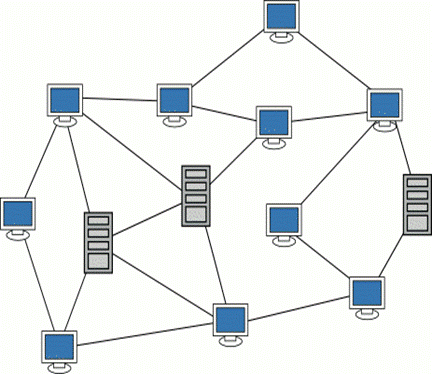
\includegraphics[scale=0.6]{mesh_topology.png}
	\end{center} \cite{IMG2}

	\noindent \\ \textbf{Advantages} of using Mesh Topology LAN Over Radio:
	\begin{itemize}
		\item All advantages listed in \textbf{Star Topology LAN Over Radio}
		\item No single choke point or point of failure in the network
	\end{itemize}

	\noindent \\ \textbf{Disadvantages} of using Mesh Topology LAN Over Radio:
	\begin{itemize}
		\item Taking BATMAN for example, it is relatively new and not in wide-spread use.  Further research is needed into implementation.
		\item Set up time is significantly longer than traditional star topology based networks (must be done manually).
		\item Configuring devices to use this network type along side traditional networks can also be a hassle.
	\end{itemize}


	\subsection{Discussion}
	All of these technologies will connect clients to the hosted web interface, but not all of them meet the criteria for simplicity.
	Using a star architecture, one can eliminate any extra setup time, because most devices are already programmed for "plug n' play" on this topology.
	This topology also allows changes to the network to be made easily and quickly.
	This entire network is not going to be extremely complex either.  The project is not aiming for thousands or even hundreds of clients.
	At a maximum, a distributed system in a greenhouse could be comprised of up to 20 controllable beds, each hosting their own interface.
	(This considers a moderate sized greenhouse found at common private nurseries that sell to the public.) 	The project has envisioned multiple levels of systems,
	but none of these levels cannot be achieved by the simplest of the three network types.  All three could handle every requirement, except simplicity in some cases.

	\subsection{Conclusion}
	Due to the need for simplicity of setup, a star type topology is going to be the network architecture used.
	Because most network infrastructure devices can integrate both wired and wireless device, the end network may see a mix of wireless and wired clients.
	For iteration beginnings and the need for even further simplicity to develop on, the team will most likely start with wired connections.



\section{Custom Enclosure Design}

	\subsection{Overview and Criteria}
	Looking further forward and at further research, vertical lighting and a custom enclosure provide even better growing conditions for the plants.  The enclosure should
	be able to house the plants, soil, the main controller, a slave microcontroller, and the ramparts or verticals that would hold the LED strips.  Still conforming to the
	requirements of simplicity, the design must be affordable, and quick to acquire.  The design must also be able to change as the user sees fit, due to possibly changing
	conditions such as different plants and placement of the enclosure.

	\subsection{Potential Candidates}
	Because there are many options when designing something mechanical in nature, the following options were produced because of their popularity and widespread use.  The
	first option the team explored was 3D printing the necessary hardware for the enclosure.  The second option was simply finding and recommending, or ourselves designing
	pre-fabricated parts to make up the planter beds, that the end user could purchase.  The third option considered was a design involving temporary adhesive connections.

	\subsubsection{3D Printed Hardware}
	In the past few years, 3D printing has exploded as a hobby, and as a practical manufacturing technique for quick, impromptu, custom hardware.  3D printing involves 3D
	generation and rendering of 3d objects in modeling software.  The files created by such modeling software can then be printed.  The printing process involves a printer
	head that moves in the X and Y dimensions, and a printing table that moves up and down in the Z dimesions.  Most printers print a rigid plastic that is heated to
	melting temperatures, and then laid down on the printer table to form layers that make up the 3D object.

	\begin{center}
		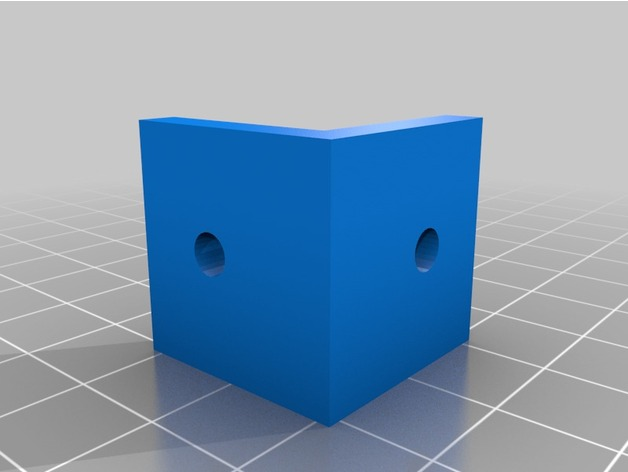
\includegraphics[scale=0.5]{90-degree-bracket.jpg}
	\end{center} \cite{IMG3}

	\noindent \\ \textbf{Advantages} of 3D printing parts for a planter bed:
	\begin{itemize}
		\item Relatively inexpensive compared to other methods or purchasing hardware
		\item If source files provided, 3D printing allows end users to customize the hardware if necessary
		\item Could potentially be quicker to print ones own custom parts, rather than custom order them
	\end{itemize}

	\noindent \\ \textbf{Disadvantages} of 3D printing parts for a planter bed:
	\begin{itemize}
		\item The client might have to learn how to use a 3D printer and 3D modeler, adding complexity.
		\item Hardware may not be printed correctly or could be not as strong as something professionally manufactured.
		\item Hardware may take some a long time to print, depending on what is printed
	\end{itemize}

	\newpage % A better place to break and transition to new page

	\subsubsection{Pre-Fabricated}
	If one is not able to create their own hardware for the planter box, then they might look to someone or a company that could.  Thus, an external source is
	required to make the parts for the end users to most likely purchase.  These pieces of hardware would be professionally created, and often free from
	defect.  The team would be able to recommend parts to the end user, and prepare a simple setup guide to follow to assemble the manufactured parts.

	\noindent \\ \textbf{Advantages} of Pre-Fabricating Parts:
	\begin{itemize}
		\item Client sets up the beds with a simple guide
		\item Client doesn't have to wait on parts to be made
		\item Client doesn't have to make their own parts
	\end{itemize}

	\noindent \\ \textbf{Disadvantages} of Pre-Fabricating Parts:
	\begin{itemize}
		\item Client may not be able to customize the parts to a custom enclosure of their own
		\item Client could end up paying more than other methods
		\item Adds another design implementation to the \textit{software developer's} list (team does not consist of any machinists or mechanical engineers)
	\end{itemize}


	\subsubsection{"Slap On"-type Connections}
	As the name conveys, this option allows one to simply put together parts in a somewhat naïve fashion.  Through the use of adhesive tapes or more structurally sound glues,
	one is able to connect parts by simply putting them face to face, with the adhesive between holding them together.  The adhesive may be a long term hold like epoxy, or a
	short term hold such as two-sided foam tape.

	\noindent \\ \textbf{Advantages} of "Slap On"-type Connections:
	\begin{itemize}
		\item The least expensive option provided.  Easy to get replacements.
		\item The easiest to assemble and disassemble, this option stands out for mobility purposes.
	\end{itemize}

	\noindent \\ \textbf{Disadvantages} of "Slap On"-type Connections:
	\begin{itemize}
		\item "You get what you pay for." Items are not durable.
		\item Connections may not hold permanently or are insecure.  Electrical connections might suffer at this option.
		\item Connections may not hold at all, and planter beds may fall apart depending on weight forces.
	\end{itemize}


	\subsection{Discussion}
	Seeing that this section doesn't quite have a coding or electical design to it, not much time was spent on developing options.  The options considered were found to be the
	simplest.  Of the three, the least cost and effort would go towards the "Slap-On" method.  However cheap and easy it may be, this option may prove not to have the structural
	integrity that the application requires.  Designing parts to have fabricated is an option that likely would not be implemented, but it is not out of the question.  This option
	adds an exteme layer of simplicity for the end user, who would basically have to follow a simple instruction set to assemble said parts.  However, the team doesn't have a
	mechanical or civil engineering background, and further research or collaboration with outside sources would be required to complete this implementation.  The last option of
	3D printing the parts necessary offers the argument of being simple to produce, relatively inexpensive, and customizable.

	\subsection{Conclusion}
	Due to the factors that the enclosure must be simple to create and modify, the team has opted to use 3D printed parts as the viable solution.  This is because of current knowledge
	levels of the team to be able to manufacture parts, the simplicity of the method, and the increasing reliability of 3D printers.  This option also features the structurally integrity
	that the planter box will require.  Since this section is part of the stretch goals of the project, simplicity and cost force the choice of this option.

	\newpage % A better place to break and transition to new page

	\section{Control Service Language}

		\subsection{Overview and Criteria}
		The Control Service will be the main program that interfaces between the Web Interface and the microcontrollers driving the RGB LEDs.  It doesn't necessarily need to be simple
		for the end user, since they may not ever need to interact with it.  However, it should be simple enough for the team to understand, so that development and bug squashing comes
		easier.  The language that the Control Service is written in, will play a crucial part in development and testing.  This language is also restricted to the particular hardware
		that will be used in the project.  If a Raspberry Pi is used as the main microcontroller, it will not be able to run languages that are process or memory intensive.

		\subsection{Potential Candidates}
		Heavily based upon the restrictions of hardware, the team has selected the following programming languages.  The first option is the widely used and persistent C/C++ language.
		The second option considered was a language that closely mimics the language used to write the web interface control.  The third and final option was Rust, a new member of the
		C++ family.

		\subsubsection{C/C++}
		The C language has been around since the early 1970s. \cite{LANG1}  It is extremely powerful compared to other languages because it is one of the few languages that comes closely
		to mimicing Assembly, a very low level microprocessor instruction language.  This means that when compiled, the code produces an efficient executing program.  Efficient in the terms
		that the processor can do the most in the least amount of time, with the least amount of memory. Considering these ideologies, the UNIX and *nix family of operating systems
		foundations are built on this language.  From C sprouted C++, which essentially is the same core language.  The only difference between the two is that C++ was developed to support Object Oriented (OO) programming.  C++ programming has the caveats of
		being based on the C language while incorporating the powerful idea of objects in a programming language.

		\noindent \\ \textbf{Advantages} of using C/C++:
		\begin{itemize}
			\item Extremely fast execution
			\item Lightweight in memory
			\item Small and efficient enough to run on the most basic microprocessors
			\item The team is already familiar with the language due to previous use
			\item The LED strips and their already developed libraries are based on C/C++
			\item Documentation and examples for these languages are nearly endless
		\end{itemize}

		\noindent \\ \textbf{Disadvantages} of using C/C++:
		\begin{itemize}
			\item The language is somewhat restrictive on syntax and operation
		\end{itemize}


		\subsubsection{Web Based Language(NodeJS, PHP, etc)}
		Considering that the main front facing interface between the user and the LEDs will be a Web Interface, the language that this interface is written in must be considered to operate
		the Control Service.  NodeJS or PHP would be two choices for the language selected to drive the front end.

		\noindent \\ \textbf{Advantages} of using Web Based Language:
		\begin{itemize}
			\item Front end that the user sees is written in the same languages
			\item Reduces number of languages used through the project
		\end{itemize}

		\noindent \\ \textbf{Disadvantages} of using Web Based Language:
		\begin{itemize}
			\item Interfacing with the microcontoller driving the LEDs would be extremely difficult (most Web languages never have to pass serial to a microcontoller)
			\item The language may not have the proper process control compared to languages that drive operating systems or other small microcontrollers
			\item The language may not run efficiently on the smaller microcontroller when trying to perform the necessary operations of the Control Service.
		\end{itemize}


		\subsubsection{Rust}
		A relatively new language, Rust is basically a child of C++.  While being syntactically very similar to C++, Rust claims to have better memory managment, and also be developed with the
		sense that the language should maintain system functionality.  Rust has grown to be a new choice for operating systems, game engines, and even virtual reality applications. \cite{LANG2}

		\noindent \\ \textbf{Advantages} of using Rust:
		\begin{itemize}
			\item Light on memory and processing
			\item Newer language means potential for new features, specifically object controller
			\item Lots of documentation on the language
		\end{itemize}

		\noindent \\ \textbf{Disadvantages} of using Rust:
		\begin{itemize}
			\item Being a relatively new language, the team has not had experience with it.
			\item For the same reason above, the documentation specific to the project application or its hardware may not exist.
			\item Rust does have very strict coding practices, that may not be enforceable on the selected hardware.
		\end{itemize}


		\subsection{Discussion}
		Looking further into the requirements for the project, the LED strips have to be driven with a library of some sort that has been developed with C or C++.  Thus, being written in a OS
		type language, the team should be able to implement the same features or applications of the libraries into the Control Service.  C/C++ is also very efficient compared to NodeJS or PHP.
		These specific Web languages also do not have the immediate capabilities to interface with a microcontroller to update the LEDs.  Rust does have its caveats in being new and efficient
		at the same time, but adaptation and adoption of this new language might prove challenging while a simpler solution exists.

		\subsection{Conclusion}
		The team has selected C++ to be the lead language in the Control Service.  It's relativeness to the LED libraries that drive the hardware, combined with the team's knowledge on it and
		the efficiency of the language, it presents itself as the clear front runner.  It clearly meets every requirement laid out by the team, and currently has too little drawbacks to be replaced
		by another of the proposed languages.


	\section{Weekly Blog Posts}
		\subsection{Austin Hodgin}
		\subsection{Travis Hodgin}
		\subsection{Zach Lerew}
		\subsection{Max Schmidt}

	\section{Final Poster}
	% 8.5 X 11 formatted, landscape

	\section{Project Documentation}
	% How does your project work? (Could include the following...)
	% What is its structure?
	% What is its Theory of Operation?
	% Block and flow diagrams are good here.
	% How does one install your software, if any?
	% How does one run it?
	% Are there any special hardware, OS, or runtime requirements to run your software?
	% Any user guides, API documentation, etc.
	% This needs to be detailed enough to recreate and/or use your project!

	\section{Recommended Technical Resources}
	% What web sites were helpful? (Listed in order of helpfulness.)
	% What, if any, reference books really helped?
	% Were there any people on campus that were really helpful?

	\section{Reflection}
		\subsection{Austin Hodgin}
			\subsubsection{What technical information did you learn?}
			\subsubsection{What non-technical information did you learn?}
			\subsubsection{What have you learned about project work?}
			\subsubsection{What have you learned about project management?}
			\subsubsection{What have you learned about working in teams?}
			\subsubsection{If you could do it all over, what would you do differently?}
		\subsection{Travis Hodgin}
			\subsubsection{What technical information did you learn?}
			\subsubsection{What non-technical information did you learn?}
			\subsubsection{What have you learned about project work?}
			\subsubsection{What have you learned about project management?}
			\subsubsection{What have you learned about working in teams?}
			\subsubsection{If you could do it all over, what would you do differently?}
		\subsection{Zach Lerew}
			\subsubsection{What technical information did you learn?}
			\subsubsection{What non-technical information did you learn?}
			\subsubsection{What have you learned about project work?}
			\subsubsection{What have you learned about project management?}
			\subsubsection{What have you learned about working in teams?}
			\subsubsection{If you could do it all over, what would you do differently?}
		\subsection{Max Schmidt}
			\subsubsection{What technical information did you learn?}
			\subsubsection{What non-technical information did you learn?}
			\subsubsection{What have you learned about project work?}
			\subsubsection{What have you learned about project management?}
			\subsubsection{What have you learned about working in teams?}
			\subsubsection{If you could do it all over, what would you do differently?}
	\section{Conclusion}


	%%% References %%%
	\subsection*{References}
	\begingroup
		\renewcommand{\addcontentsline}[3]{}% Remove functionality of \addcontentsline
		\renewcommand{\section}[2]{}% Remove functionality of \section
		%\cite[Sec 3.8]{sourceName}
		\bibliography{ref}
		\bibliographystyle{IEEEtran}
	\endgroup
\end{document}
